\documentclass[a4paper]{book}

\usepackage{amsmath}
\usepackage{amssymb}
\usepackage{array}
\usepackage{graphicx}
\usepackage{hyperref}
\usepackage{listings}
\usepackage{longtable}
\usepackage{natbib}
\usepackage{nicefrac}
\usepackage{ulem}

\newcommand{\pequod}{PEQUOD}
\newcommand{\pequodexpanded}{Parallel Quasi-Geostrophic Model}
\newcommand{\version}{0.9.5-dev}

\begin{document}

\begin{titlepage}
\begin{center}

\Huge{\pequod\ Manual} \\[0.02\textheight]
\large{\pequodexpanded} \\[0.02\textheight]
\Huge{Version \version} \\[0.15\textheight]
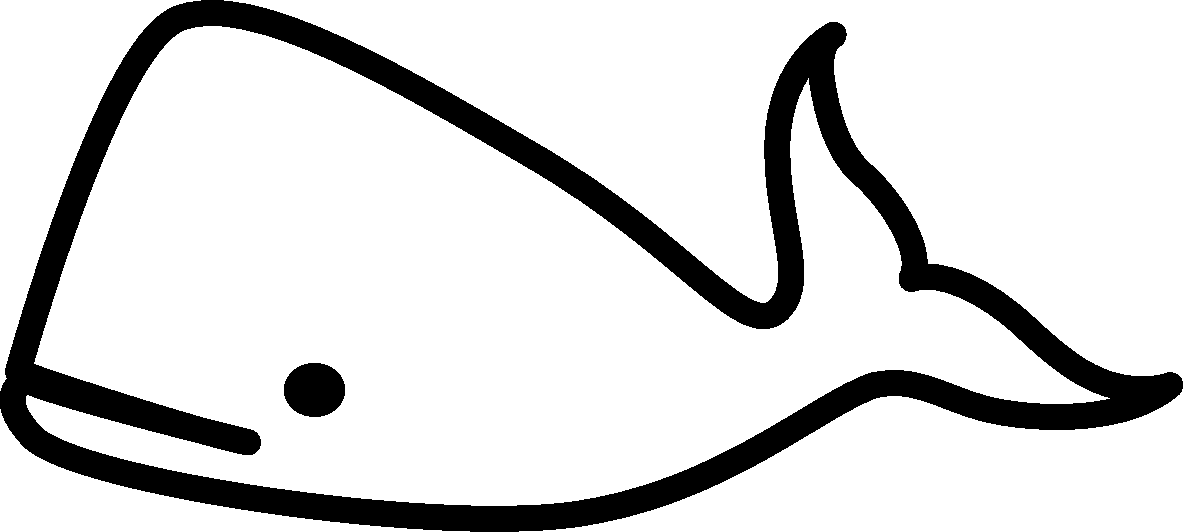
\includegraphics[width=0.4\textwidth]{figs/stumbles_Whale.pdf} \\[0.3\textheight]
\Large{Dr. J. R. Maddison, Dr. P. S. Berloff, \\ Dr. S. A. Karabasov} \\[0.15\textheight]
\vfill
\large{\today}

\end{center}
\end{titlepage}

\tableofcontents

\chapter*{Symbols and notation}

\setlength{\extrarowheight}{3pt}
\begin{center}
\begin{longtable}{ | c | p{0.7\textwidth} | }
  \hline
  Symbol               & Definition \\
  \hline
  \endhead
  \hline
  \endfoot
  $\partial_X$         & Partial differentiation with respect to a variable
                         $X$. \\
  $D_t$                & Material, or advective, derivative. \\
  $\uline{\nabla}_H$   & Two dimensional horizontal del operator. \\
  $J(X, Y)$            & Determinant of the two dimensional Jacobian matrix
                         formed by $X$ and $Y$, $J(X, Y) = \partial_x X
                         \partial_y Y - \partial_y X \partial_x Y$. \\
  $\delta \left( \ldots \right)$  & Dirac delta function. \\
  $\uline{X}$          & Vector. \\
  $X_i$                & $i$th element of a vector $\uline{X}$. \\
  $\uuline{X}$         & Matrix. \\
  $X_{ij}$                & $i,j$th element of a matrix $\uuline{X}$. \\
  $\uuline{I}$         & Identity matrix. \\
  $\delta_{ij}$        & Kronecker delta, $I_{ij} = \delta_{ij}$. \\
  \hline
  $x$                  & Zonal coordinate. \\
  $y$                  & Meridional coordinate. \\
  $z$                  & Vertical coordinate. \\
  $q$                  & Quasi-geostrophic potential vorticity (or ``potential
                         vorticity''). \\
  $\zeta$              & Relative quasi-geostrophic potential vorticity (or
                        ``relative potential vorticity''). \\
  $\omega$             & Relative vorticity. \\
  $\psi$               & Quasi-geostrophic stream function (or ``stream
                         function''). \\
  $\rho$               & Fluid density. \\
  $\rho_0$             & Fluid reference density. \\
  $u$                  & Zonal velocity (at zeroth order in Rossby number). \\
  $v$                  & Meridional velocity (at zeroth order in Rossby
                         number). \\
  $b$                  & Buoyancy (at zeroth order in Rossby number). \\
  $w_a$                & Vertical velocity (at first order in Rossby
                         number). \\
  \hline
  $f$                  & Planetary vorticity. \\
  $f_0$                & Typical planetary vorticity at domain mid-$y$. \\
  $\beta$              & Meridional planetary vorticity gradient. \\
  $g$                  & Gravitational acceleration. \\
  $g'$                 & Reduced gravity. \\
  $\nu$                & Coefficient of Laplacian viscosity for momentum. \\
  $r$                  & Bottom drag coefficient. \\
  $\tau$               & Wind stress per unit density. \\
  $F$                  & Forcing and dissipation terms in the quasi-geostrophic
                         potential vorticity equation. \\
  \hline
  $\uuline{S}$         & Stratification matrix. \\
  $\uuline{D}$         & Diagonalisation matrix for $\uuline{S}$, such that
                         $\uuline{D}~\uuline{S}~\uuline{D}^{-1} =
                         \uuline{\lambda}$. \\
  $\uuline{\lambda}$   & Matrix of eigenvalues of $\uuline{S}$,
                         $\lambda_{ij} = \delta_{ij} l_i$ where $l_i$
                         is the $i$th eigenvalue for $\uuline{S}$. \\
  $R_{D,i}$            & Rossby radii of deformation. \\
  $\uuline{A}_i$       & Advection matrix for $i$th baroclinic mode. \\
  $\tilde{\uline{X}}$  & Baroclinic modal projection of a layer variable
                         $\uline{X}$. $\tilde{\uline{X}} =
                         \uuline{D}~\uline{X}.$ \\
  \hline
  $\Delta x$           & Grid spacing. \\
  $\Delta t$           & Time step size. \\
  $N_i$                & Number of grid points in the zonal direction. \\
  $N_j$                & Number of grid points in the meridional direction. \\
  $X_{i,j}$            & Value of a quantity $X$ at grid point $i$ in the
                         zonal direction and $j$ in the meridional direction. \\
  $X^n$                & Value of a quantity $X$ at time level $n$. \\
  $\nu$                & Robert-Asselin filter parameter. \\
  $\gamma$             & Robert-Asselin-Williams (RAW) filter parameter. \\
  \hline
\end{longtable}
\end{center}

\chapter{Introduction}

\pequod\ (the \pequodexpanded) is a finite difference code for
solving the multi-layer quasi-geostrophic equations in a rectangular domain. The
model has two primary modes of operation: basin mode and channel mode.
Typically, the basin mode is used as a simple model for a wind driven double
gyre, with energy input to the system via upper layer wind forcing. The channel
mode is used as a simple model for baroclinic zonal jet formation, with the
energy input to the system via lateral buoyancy forcing.

\pequod\ is primarily intended for the study of mesoscale eddy processes. To
this end, \pequod\ implements the advanced CABARET scheme (the Compact
Accurately Boundary Adjusting high-REsolution Technique), a form of second-order
upwind scheme implementing a non-linear flux limiter. The model is fully
parallelised using MPI. The combination of the high-resolution and stable
CABARET scheme, together with MPI parallelism, makes \pequod\ suitable for high
resolution eddy resolving numerical simulations in which multiple baroclinic
deformation radii are fully resolved.

\chapter{Model equations}

In this chapter the equations solved by \pequod\ are outlined. The
quasi-geostrophic potential vorticity equation is introduced in section
\ref{sect:qgpv}. The modification of this equation in the presence of a
background vertical shear is discussed in section \ref{sect:shear}, and the
boundary conditions stated in section \ref{sect:qgpv_bc}. The level and layer
formulations are described in section \ref{sect:qgpv_layered}, and the
projection onto vertical modes is described in section \ref{sect:qgpv_modal}.
Finally, forms of forcing and dissipation are stated in section
\ref{sect:qgpv_forcing}.

\section{Quasi-geostrophic potential vorticity equation}\label{sect:qgpv}

\pequod\ solves the quasi-geostrophic potential vorticity equation subject
to forcing and dissipation. These equations arise from an asymptotic expansion
of the momentum, mass continuity and thermodynamic equations, retaining
terms up to first order in Rossby number. Only the key results are listed here.
For a complete derivation, see \citet{pedlosky1987} and \citet{vallis2006}.

At leading order in Rossby number we have geostrophic and hydrostatic balance:
\begin{align}
  u = -\partial_y \psi, & & v = \partial_x \psi, & & w = 0, & & b = f_0 \partial_z \psi,
\end{align}
where $u$, $v$, $w$, and $b$ are the zeroth order contributions for the
zonal velocity, meridional velocity, vertical velocity, and buoyancy
respectively, and $\psi$ is the quasi-geostrophic stream function (hereafter
referred to as the ``stream function''). At next order in Rossby number
one obtains the quasi-geostrophic potential vorticity equation:
\begin{equation}\label{eqn:qgpv_equation}
  D_t q = F,
\end{equation}
where $q$ is the quasi-geostrophic potential vorticity (hereafter referred to as
the ``potential vorticity''), $D_t = \partial_t + J(\psi, q)$ is the
material derivative, and $F$ is any forcing and dissipation. The advection term
is defined using the leading order horizontal velocity, and notated in terms of
the determinant of the horizontal Jacobian matrix formed by $\psi$ and $q$:
\begin{align}
  J(\psi, q) & = \left| \begin{array}{cc}\partial_x \psi & \partial_x q \\ \partial_y \psi & \partial_y q \end{array}\right|  \nonumber \\
             & = \partial_x \psi \partial_y q - \partial_y \psi \partial_x q \nonumber \\
             & = \uline{u} \cdot \uline{\nabla}_H q,
\end{align}
where $\nabla_H$ is the horizontal del operator and
$\uline{u} = \left( u, v \right)$. The potential vorticity is given by:
\begin{equation}\label{eqn:qgpv}
  q = \nabla^2 \psi + \beta y + \partial_z \left( \frac{f_0^2}{N^2} \partial_z \psi \right),
\end{equation}
where $f = f_0 + \beta y$ is the planetary vorticity subject to the
$\beta$-plane approximation and $N$ is the buoyancy frequency. The first term
in equation \eqref{eqn:qgpv} is the relative vorticity, the second term is the
contribution due to the background vorticity gradient (arising from the
planetary vorticity), and the third term is the contribution due to the vertical
buoyancy gradient (the ``thickness'' term).

\section{Background vertical shear}\label{sect:shear}

Let $0 \leq z \leq H$, and let the stream function be given by:
\begin{equation}
  \psi = -\frac{U y z}{H} + \psi'.
\end{equation}
This is equivalent to a vertical shear in the $x$-direction, from a velocity of
zero at the lower boundary to a velocity of $U$ at the upper boundary, and with
a deviation of $\psi'$ from the background shear. The potential vorticity \eqref{eqn:qgpv}
becomes:
\begin{align}
  q & = \nabla^2 \psi' + \beta y + \partial_z \left( \frac{f_0^2}{N^2} \partial_z \psi' \right) - \frac{U y}{H} \partial_z \left( \frac{f_0^2}{N^2} \right) \nonumber \\
    & = \nabla^2 \psi' + \tilde{\beta} y + \partial_z \left( \frac{f_0^2}{N^2} \partial_z \psi' \right),
\end{align}
where $\tilde{\beta} = \beta -  \frac{U}{H} \partial_z \left( \frac{f_0^2}{N^2} \right)$. The potential vorticity
equation \eqref{eqn:qgpv_equation} becomes:
\begin{equation}
  \partial_t q + J \left( \psi', q \right) + \frac{U z}{H} \partial_x q =  F.
\end{equation}
Hence the presence of a background vertical shear is equivalent to a
modification of the background vorticity gradient, combined with an additional
linear advection of potential vorticity.

\section{Boundary conditions}\label{sect:qgpv_bc}

The quasi-geostrophic thermodynamic equation is:
\begin{equation}
  D_t b + N^2 w_a = 0,
\end{equation}
where $w_a$ is the first order (in Rossby number) contribution for the vertical
velocity (and the advection is by the leading order, geostrophic velocity).
Applying free-slip boundary conditions at the upper and lower
boundaries yields the boundary condition:
\begin{equation}\label{eqn:qgpv_bc}
  D_t b = f_0 D_t \partial_z \psi = 0 \quad \textrm{on} \quad \partial \Omega_U \cup \partial \Omega_B,
\end{equation}
where $\partial \Omega_U$ and $\partial \Omega_B$ are the upper and lower
boundaries respectively. Note that, in the presence of Ekman boundary layers,
the right-hand size of \eqref{eqn:qgpv_bc} becomes non-zero.

Equivalently, following \citet{bretherton1966}, the boundary condition
\eqref{eqn:qgpv_bc} may be replaced by the homogeneous boundary condition :
\begin{align}\label{eqn:bm_qgs}
  \psi \rightarrow \psi^*, \quad \partial_z \psi^* = 0 \quad \textrm{on} \quad \partial \Omega_U \cup \partial \Omega_B,
\end{align}
provided the potential vorticity \eqref{eqn:qgpv} is modified to:
\begin{align}\label{eqn:bm_qgpv}
  q \rightarrow q^* & = \nabla^2 \psi^* + \beta y + \partial_z \left( \frac{f_0^2}{N^2} \partial_z \psi^* \right) \nonumber \\
                    & = \nabla^2 \psi + \beta y + \partial_z \left( \frac{f_0^2}{N^2} \partial_z \psi \right) + q^*_B,
\end{align}
where:
\begin{equation}
  \int_{z - \delta z}^{z + \delta z} q^*_B dz' = \left\{
                                                   \begin{array}{l l}
                                                     + \left. \left( \frac{f_0}{N^2} b \right) \right|_{H_B} & \textrm{if } H_B \in \left[ z - \delta z, z + \delta z \right] \\
                                                     - \left. \left( \frac{f_0}{N^2} b \right) \right|_{H_U} & \textrm{if } H_U \in \left[ z - \delta z, z + \delta z \right] \\
                                                     + \left. \left( \frac{f_0}{N^2} b \right) \right|_{H_B} - \left. \left( \frac{f_0}{N^2} b \right) \right|_{H_U} & \textrm{if } H_B, H_U \in \left[ z - \delta z, z + \delta z \right] \\
                                                     0                                                  & \textrm{otherwise},
                                                   \end{array}
                                                \right.
\end{equation}
where $H_U$ and $H_B$ are the $z$-coordinates of the upper and lower boundaries
respectively. With some abuse of notation \eqref{eqn:bm_qgpv} can be expressed
via:
\begin{align}
  q \rightarrow q^* = \nabla^2 \psi + \beta y + \partial_z \left( \frac{f_0^2}{N^2} \partial_z \psi \right) \qquad \qquad \qquad \qquad \qquad \qquad \nonumber \\
    + \lim_{\epsilon \rightarrow 0^+} \left[ \frac{f_0}{N^2} b \left[ \delta (z - H_B + \epsilon) - \delta (z - H_U - \epsilon) \right] \right].
\end{align}
Note that $b^* = f_0 \partial_z \psi^* = b = f_0 \partial_z \psi$ only in the
open interval $\left( H_B, H_U \right)$. See \citet{schneider2003} for the
origins of this boundary modified potential vorticity from the
non-quasi-geostrophic case.

Restated, the potential vorticity equation \eqref{eqn:qgpv_equation} with
a potential vorticity of the form \eqref{eqn:qgpv}, combined
with the boundary condition \eqref{eqn:qgpv_bc}, is (neglecting forcing and
dissipation and Ekman boundary layers) a statement of material conservation
of potential vorticity in the interior and material conservation of buoyancy on the
upper and lower boundaries. It follows that this can be combined to a statement
of material conservation of a single quantity, the boundary modified potential
vorticity \eqref{eqn:bm_qgpv}. This mathematical construction permits
flow constraints and stability criteria to be formulated only in terms of the
boundary modified potential vorticity.

\section{Layered quasi-geostrophic potential vorticity equation}\label{sect:qgpv_layered}

We consider a finite difference discretisation of equation
\eqref{eqn:qgpv_equation} in the vertical dimension using centred finite
differencing. Divide the vertical dimension into $N$ levels and let the
$i$th level have thickness $h_i$. Apply second order centred finite differencing
in the vertical, subject to the boundary condition $\partial_z \psi = 0$ on the
upper and lower boundaries. This choice of boundary condition is appropriate,
provided we recognise that the potential vorticity has been substituted
with the boundary modified potential vorticity as per equation
\eqref{eqn:bm_qgpv}. The boundary terms in \eqref{eqn:bm_qgpv} provide a
contribution to the upper- and lowermost levels.

The equation for the potential vorticity \eqref{eqn:qgpv} becomes:
\begin{equation}\label{eqn:zeta_layered}
  \uline{\zeta} = \nabla^2 \uline{\psi} + \uuline{S}~\uline{\psi},
\end{equation}
where $\zeta = q - \beta y$ is the relative potential vorticity,
$\uline{\zeta}$ and $\uline{\psi}$ are vectors defining the relative potential
vorticity and stream function in each level, and $\uuline{S}$ is a stratification matrix.
The stratification matrix $\uuline{S}$ is defined such that, assuming $N \ge 2$:
\begin{equation}
  \sum_{j = 1}^{N} S_{ij} \psi_j = \left\{ \begin{array}{l l}s_1^{+} \left( \psi_2 - \psi_1 \right)                                                     & \quad \textrm{if} \quad i = 1, \\
                                                           s_i^{-} \left( \psi_{i - 1} - \psi_i \right) + s_i^{+} \left( \psi_{i + 1} - \psi_i \right)  & \quad \textrm{if} \quad 1 < i < N, \\
                                                           s_N^{-} \left( \psi_{N - 1} - \psi_N \right)                                                 & \quad \textrm{if} \quad i = N,
                                           \end{array} \right.
\end{equation}
where:
\begin{align}\label{eqn:stratification_parameters}
  s_i^{-} = \frac{f_0^2}{N_{i - \nicefrac{1}{2}}^2} \frac{2}{h_i \left( h_{i - 1} + h_i \right)}, \nonumber \\
  s_i^{+} = \frac{f_0^2}{N_{i + \nicefrac{1}{2}}^2} \frac{2}{h_i \left( h_{i + 1} + h_i \right)},
\end{align}
and where $N_{i - 1 / 2}$ is buoyancy frequency at the interface
between the $\left( i - 1 \right)$ and $i$th levels, and $N_{i + 1 / 2}$ is the
buoyancy frequency at the interface between the $i$ and $\left( i + 1 \right)$th
levels. $i = 1$ and $i = N$, correspond to the upper- and lowermost levels
respectively. The quasi-geostrophic potential vorticity equation
\eqref{eqn:qgpv_equation} now becomes, for each level:
\begin{equation}\label{eqn:qgpv_layered}
  \partial_t q_i + J(\psi_i, q_i) = F_i.
\end{equation}

The vertically discretised level model \eqref{eqn:qgpv_layered}
with relative potential vorticity \eqref{eqn:zeta_layered} is
mathematically equivalent to a number of stacked quasi-geostrophic shallow-water
layers \citep{vallis2006}. In such a layer model the interfacial buoyancy frequencies
are replaced by:
\begin{align}
  N_{i - \nicefrac{1}{2}}^2 = \frac{2 g_{i - \nicefrac{1}{2}}'}{\left( h_{i - 1} + h_i \right)}, \nonumber \\
  N_{i + \nicefrac{1}{2}}^2 = \frac{2 g_{i + \nicefrac{1}{2}}'}{\left( h_{i + 1} + h_i \right)}, \nonumber
\end{align}
where $g_{i - 1 / 2}'$ is the reduced gravity between the $i - 1$ and
$i$th layers, and $g_{i + 1 / 2}'$ is the reduced gravity between the
$i + 1$ and $i$th layers, where:
\begin{align}
  g_{i - \nicefrac{1}{2}}' = -g \frac{\rho_{i - 1} - \rho_i}{\rho_0}, \nonumber \\
  g_{i + \nicefrac{1}{2}}' = -g \frac{\rho_i - \rho_{i + 1}}{\rho_0},
\end{align}
where $g$ is the gravitational acceleration, $\rho$ are the densities in each
layer, and $\rho_0$ is a reference density.

Note that a second order finite volume discretisation in the vertical also
yields the level formulation \eqref{eqn:qgpv_layered}, making clear the
equivalence between the level and layer formulations.

\section{Modal quasi-geostrophic potential vorticity equation}\label{sect:qgpv_modal}

Multiplying equation \eqref{eqn:zeta_layered} by some matrix $\uuline{D}$
yields:
\begin{equation}\label{eqn:zeta_d}
  \uuline{D}~\uline{\zeta} = \nabla^2 \uuline{D}~\uline{\psi} + \uuline{D}~\uuline{S}~\uline{\psi}.
\end{equation}
We now choose $\uuline{D}$ such that:
\begin{equation}\label{eqn:s_diagonalisation}
  \uuline{D}~\uuline{S}~\uuline{D}^{-1} = \uuline{\lambda} ,
\end{equation}
where $\uuline{\lambda}$ is a diagonal matrix. This defines an eigenvalue
problem for $\uuline{S}$ \citep{strang1988}, and it follows that $\uuline{D}^{-1}$ is a matrix whose columns are the
eigenvectors of $\uuline{S}$ and the diagonal entries of $\uuline{\lambda}$
are the corresponding eigenvalues. Hence equation \eqref{eqn:zeta_d} becomes:
\begin{equation}
  \uuline{D}~\uline{\zeta} = \nabla^2 \uuline{D}~\uline{\psi} + \uuline{\lambda}~\uuline{D}~\uline{\psi},
\end{equation}
yielding a series of decoupled Helmholtz equations:
\begin{equation}\label{eqn:zeta_modal}
  \tilde{\zeta}_i = \left( \nabla^2 + l_i \right) \tilde{\psi}_i,
\end{equation}
where, for a variable $X$, $\tilde{X}_i = \sum_{j = 1}^N D_{ij} X_j$, and where
$l_i$ is the $i$th eigenvalue of $\uuline{S}$.

Equation \eqref{eqn:s_diagonalisation} is the vertically
discretised eigenvalue problem for the vertical structure functions in
a decomposition of the system in terms of vertical modes (compare with equation
(6.12.7a) of \citet{pedlosky1987}). It follows that
the corresponding eigenvalues $l_i$ are defined in terms of the Rossby
radii of deformation, $R_{D,i}$:
\begin{equation}
  l_i = -\frac{1}{R_{D,i}^2}.
\end{equation}
Hence $\tilde{X}_i$ denotes $X$ for the $i$th baroclinic mode. Note that provided
the deformation radii are distinct, it follows that $\uuline{D}^{-1}$ is
invertible \citep{strang1988}. Hereafter, the barotropic mode (with $R_D = \infty$)
is associated with $i = 1$, and the remaining modes (the baroclinic modes)
with $i \geq 2$.

The quasi-geostrophic potential vorticity equation \eqref{eqn:qgpv_equation}
now becomes, for each mode:
\begin{equation}\label{eqn:qgpv_equation_modal}
  \partial_t \tilde{q}_i + \sum_{i = j}^N \sum_{j = k}^N A_{ijk} J \left( \tilde{\psi}_j, \tilde{q}_k \right) = \tilde{F}_i,
\end{equation}
where:
\begin{equation}
  A_{ijk} = \sum_{l = 1}^N D_{il} D^{-1}_{lj} D^{-1}_{lk}.
\end{equation}

\section{Forcing and dissipation}\label{sect:qgpv_forcing}

A wind forcing applied to the uppermost layer takes the form:
\begin{equation}
  F_{W,i} = \delta_{i1} \frac{\left( \nabla_H \times \tau \right)_z}{h_1},
\end{equation}
where $\left( \nabla_H \times \tau \right)_z$ is the vertical component of the
wind stress curl per unit density, and $\tau$ is the wind stress per unit
density.

We consider two forms of dissipation:
\begin{equation}
  F_{D,i} = \nu \nabla^4 \psi_i - r \delta_{iN} \nabla^2 \psi_i.
\end{equation}
The fourth order term is equivalent to Laplacian viscosity for momentum, and
acts to dissipate small scale enstrophy, $q^2$, from the system. The second order
term, applied only to the bottom-most layer, represents the presence of an Ekman layer.
$\nu$ is a viscosity coefficient and $r$ is a bottom drag coefficient.

Note that the fourth order term results in an additional boundary condition
requirement. The system can be closed via a Dirichlet boundary condition for
$\nabla^2 \omega$, where $\omega = \nabla^2 \psi$ is the relative
vorticity. One such boundary condition is partial-slip which, for a boundary
aligned parallel to the $y$-axis and at $x = x_L$, takes the form:
\begin{equation}\label{eqn:partial_slip}
  \omega \left( x = x_L \right) = \left. \partial_{xx} \psi \right|_{x = x_L} = \alpha \left. \partial_x \psi \right|_{x = x_L},
\end{equation}
where $\omega = \nabla^2 \psi$ is the relative vorticity and $\alpha$ is a
partial-slip parameter (an inverse length scale associated with the
parameterised boundary layer). $\alpha \rightarrow \infty$ yields a no-slip
boundary condition, while $\alpha = 0$ yields a free-slip boundary condition.

\chapter{Numerical formulation}

\pequod\ implements two distinct numerical discretisations of the layered
quasi-geostrophic potential vorticity equation \eqref{eqn:qgpv_layered}. The
first scheme uses a centred-in-space and centred-in-time discretisation.
The second scheme utilises the Compact Accurately Boundary Adjusting
high-REsolution Technique \linebreak (CABARET), a flux limited second order upwind scheme.

Section \ref{sect:cn} describes the centred scheme, while section
\ref{sect:cabaret} describes the CABARET scheme. In these two sections it is
assumed that the stream function is available. In section
\ref{sect:pv_inversion} the method by which the potential vorticity is inverted
for the stream function is described.

\section{Centred leapfrog scheme}\label{sect:cn}

This section describes the centred leapfrog scheme. Section
\ref{sect:cn_advection} details the advection scheme, section
\ref{sect:cn_forcing} details the forcing and dissipation, section
\ref{sect:ra_filter} describes the time filter used to damp the computational
mode associated with centred differencing in time, and section \ref{sect:cn_bc}
describes the boundary conditions. Finally, section \ref{sect:cn_implementation}
describes some details associated with the implementation of this scheme by the
model.

In this section $\left( \ldots \right)_{i,j}$ denotes grid coordinate $i$ in the
zonal direction and $j$ in the meridional direction. Unless otherwise stated,
all equations are defined for $2 \leq i \leq \left( N_i - 1 \right)$ and
$2 \leq j \leq \left( N_j - 1 \right)$, where $N_i$ and $N_j$ are the number of
grid points in the zonal and meridional directions respectively.
$\left( \ldots \right)^n$ denotes time level $n$. The time step size and
grid spacing are given by $\Delta t$ and $\Delta x$ respectively.

\subsection{Advection}\label{sect:cn_advection}

In the centred leapfrog scheme the advection term is cast to flux form:
\begin{equation}
  J \left( \psi, q \right) = \nabla \cdot \left( \uline{u} q \right),
\end{equation}
where this identity holds as $\nabla_H \cdot \uline{u} = 0$. The operator is
discretised using centred differencing in space and time to yield the advection
tendency:
\begin{align}\label{eqn:cn_advection}
  \frac{q^{n + 1}_{i,j} - q^{n - 1}_{i,j}}{2 \Delta t} = & \quad \frac{1}{2 \Delta x} \left[ u^n_{i - 1,j} q^n_{i - 1,j} - u^n_{i + 1,j} q^n_{i + 1,j} \right] \nonumber \\
                                                     + & \quad \frac{1}{2 \Delta x} \left[ v^n_{i,j - 1} q^n_{i,j - 1} - v^n_{i,j + 1} q^n_{i,j + 1} \right] \nonumber \\
                                                     = & \quad \frac{1}{4 \Delta x^2} \left[ -\left( \psi^n_{i - 1,j + 1} - \psi^n_{i - 1,j - 1} \right) q^n_{i - 1,j} \right. \nonumber \\
                                                       & \qquad \qquad + \left. \left( \psi^n_{i + 1,j + 1} - \psi^n_{i + 1,j - 1} \right) q^n_{i + 1,j} \right] \nonumber \\
                                                     + & \quad \frac{1}{4 \Delta x^2} \left[ \left( \psi^n_{i + 1,j - 1} - \psi^n_{i - 1,j - 1} \right) q^n_{i,j - 1} \right. \nonumber \\
                                                       & \qquad \qquad - \left. \left( \psi^n_{i + 1,j + 1} - \psi^n_{i - 1,j + 1} \right) q^n_{i,j + 1} \right].
\end{align}
This corresponds to the discrete Jacobian $\mathbb{J}^{+\times} \left( q, \psi \right)$ in
\citet{arakawa1966}. In the model terms corresponding to
$J \left( \psi_i, \psi_i \right)$ are discarded for efficiency.

Since this is a discretisation of the potential vorticity advective flux,
potential vorticity is conserved. This method is second order accurate in space
and time.

\subsection{Forcing and dissipation}\label{sect:cn_forcing}

A time independent forcing, such as a time independent wind stress applied to
the upper layer, is discretised using centred-in-time differencing. This
leads to a tendency of:
\begin{equation}
  \frac{q^{n + 1}_{i,j} - q^{n - 1}_{i,j}}{2 \Delta t} = F_W.
\end{equation}

A stable discretisation of the tendency resulting from fourth order diffusion,
described in section \ref{sect:qgpv_forcing}, is centred differencing
in space and a simple forward Euler discretisation applied between time levels
$n - 1$ and $n + 1$:
\begin{equation}
  \frac{q^{n + 1}_{i,j} - q^{n - 1}_{i,j}}{2 \Delta t} = \frac{\nu}{\Delta x^2} \left[ \omega^{n - 1}_{i,j + 1} + \omega^{n - 1}_{i - 1,j} - 4 \omega^{n - 1}_{i,j} + \omega^{n - 1}_{i + 1,j} + \omega^{n - 1}_{i,j - 1} \right].
\end{equation}
The relative vorticity is computed using centred finite differencing:
\begin{equation}
  \omega^n_{i,j} = \frac{1}{\Delta x^2} \left[ \psi^n_{i,j + 1} + \psi^n_{i - 1,j} - 4 \psi^n_{i,j} + \psi^n_{i + 1,j} + \psi^n_{i,j - 1} \right],
\end{equation}
where the value of $\omega$ on the boundaries is determined as described in
section \ref{sect:cn_bc}. The resulting
discretisation of the fourth order diffusion term is second order
accurate in space and first order accurate in time.

Similarly, the tendency due to the second order bottom drag, as discussed in section
\ref{sect:qgpv_forcing}, is discretised using a forward Euler discretisation
between time levels $n - 1$ and $n + 1$:
\begin{equation}
  \frac{q^{n + 1}_{i,j} - q^{n - 1}_{i,j}}{2 \Delta t} = -r \omega^{n - 1}_{i,j},
\end{equation}
with second order accuracy in space and first order accuracy in time.

Note that a centred discretisation in space and time is unstable for diffusion
\citep{haltiner1980}.

\subsection{Robert-Asselin-Williams time filter}\label{sect:ra_filter}

The use of centred differencing in time is second order accurate, but a
computational mode exists which can grow over time and pollute the
resulting solution. This mode can be damped via a time filter. The time filter
used is a modified Robert-Asselin time filter as proposed by
\citet{williams2009a} -- the Robert-Asselin-Williams (RAW) filter. Centred
differencing in time for a tendency
${\cal{F}}^n \left( q^n \right)$ is modified to:
\begin{equation}
  \frac{q^{n + 1} - \overline{\overline{q}}^{n - 1}}{2 \Delta t} = {\cal{F}}^n \left( \overline{q}^n \right),
\end{equation}
where:
\begin{align}\label{eqn:modified_ra_filter}
  \overline{q}^{n + 1}        & = q^{n + 1} - \frac{\mu \left(1 - \gamma \right)}{2} \left[\overline{\overline{q}}^{n - 1} - 2 \overline{q}^n + q^{n + 1} \right], \nonumber \\
  \overline{\overline{q}}^{n} & = \overline{q}^n + \frac{\mu \gamma}{2} \left[\overline{\overline{q}}^{n - 1} - 2 \overline{q}^n + q^{n + 1} \right],
\end{align}
where $0 \leq \mu, \gamma \leq 1$. $\mu$ is a parameter controlling the strength
of the filter. For $\gamma = 1$ equation \eqref{eqn:modified_ra_filter} reduces to the
standard Robert-Asselin filter \citep{robert1966, asselin1972}, and the discretisation is
unconditionally stable and first order accurate in time. For $\gamma = 1 / 2$ the
discretisation is third order accurate in time and unconditionally unstable. For
$\gamma = 1 / 2 + \epsilon$ where $\epsilon > 0$ and $\epsilon \ll 1$ the
discretisation is quasi-third order accurate in time (although formally first
order accurate) and conditionally stable. For a full description of the modified
filter, including a derivation of the stability and accuracy properties, see
\citet{williams2009a}.

\subsection{Boundary conditions}\label{sect:cn_bc}

The fourth order diffusion term in section \ref{sect:cn_forcing}
requires an additional boundary condition for the relative vorticity $\omega$.
An appropriate boundary condition is a partial-slip Dirichlet boundary condition
(see section \ref{sect:qgpv_forcing}).

Consider a boundary aligned parallel to the
$y$-axis. Letting $i = 1$ on the boundary, a Taylor expansion retaining terms
up to third order yields:
\begin{subequations}
  \begin{equation}
    \psi_{2} = \psi_{1} + \left. \partial_x \psi \right|_{x = x_L} \Delta x + \frac{1}{2} \left. \partial_{xx} \psi \right|_{x = x_L} \Delta x^2 + \frac{1}{6} \left. \partial_{xxx} \psi \right|_{x = x_L} \Delta x^3,
  \end{equation}
  \begin{equation}
    \psi_{3} = \psi_{1} + 2 \left. \partial_x \psi \right|_{x = x_L} \Delta x + 2 \left. \partial_{xx} \psi \right|_{x = x_L} \Delta x^2 + \frac{4}{3} \left. \partial_{xxx} \psi \right|_{x = x_L} \Delta x^3.
  \end{equation}
\end{subequations}
Eliminating the third order terms and applying a partial-slip boundary condition:
\begin{equation}
  \omega_1 = \left. \partial_{xx} \psi \right|_{x = x_L} = \alpha \left. \partial_x \psi \right|_{x = x_L},
\end{equation}
yields:
\begin{equation}\label{eqn:discrete_partial_slip}
  \omega_1 = \left. \partial_{xx} \psi \right|_{x = x_L} = \frac{-7 \psi_1 + 8 \psi_2 - \psi_3}{2 \Delta x^2 + \frac{6}{\alpha} \Delta x}.
\end{equation}

Alternatively, a no-slip boundary condition can be defined via:
\begin{equation}\label{eqn:discrete_no_slip}
  \omega_1 = \left. \partial_{xx} \psi \right|_{x = x_L} = \frac{2 \psi_2 - 2 \psi_1}{\Delta x^2},
\end{equation}
which is equivalent to asserting that the tangential velocity on the boundary,
averaged between $\left( x_L + \Delta x / 2 \right)$ and an image point at
$\left( x_L - \Delta x / 2 \right)$, is zero.

Note that the boundary is defined to be co-incident with end nodes. Hence corner
cells have one quarter the area of interior cells, and other boundary cells have
one half the area of interior cells.

\subsection{Implementation details}\label{sect:cn_implementation}

\begin{enumerate}
  \item The relative potential vorticity $\zeta$ is used as the fundamental
        prognostic model variable.
  \item The advection term in the layer form of the quasi-geostrophic potential
        vorticity equation \eqref{eqn:qgpv_layered} yields terms proportional to
        $J \left( \psi_i, \psi_i \right)$. These terms are discarded for efficiency.
  \item The values of the relative potential vorticity on the boundaries are
        computed from the stream function and relative vorticity, following
        application of the boundary condition for the relative vorticity.
  \item On the first timestep a single forward Euler step of size $\Delta t$
        is used, prior to leapfrogging in time.
\end{enumerate}

\section{CABARET scheme}\label{sect:cabaret}

The second numerical method implemented in \pequod\ incorporates the
Compact Accurately Boundary Adjusting high-REsolution Technique (CABARET)
for advection of relative potential vorticity, combined with integration
of the advection of planetary vorticity and the forcing and dissipation. This
section provides a summary of the model implementation of the CABARET scheme,
and is based on \citet{karabasov2009}.

In this section $\left( \ldots \right)_{i,j}$ denotes grid coordinate $i$ in the
zonal direction and $j$ in the meridional direction.
$\left( \ldots \right)_{i + 1 / 2,j}$ denotes a point on a grid staggered in the
zonal direction, at a point between grid coordinate $i$ and $i + 1$.
$\left( \ldots \right)_{i,j + 1 / 2}$ denotes a point on a grid staggered in the
meridional direction, at a point between grid coordinate $j$ and $j + 1$.
$\left( \ldots \right)_{i + 1 / 2,j + 1 / 2}$ denotes a point on a grid
staggered in both the zonal and meridional directions.
Unless otherwise stated all equations are defined excluding points lying on the
boundary.
$\left( \ldots \right)^n$ denote time level $n$, and
$\left( \ldots \right)^{n + 1 / 2}$ denote a time level intermediate between
time levels $n$ and $n + 1$. The time step size and
grid spacing are given by $\Delta t$ and $\Delta x$ respectively.

\subsection{Advection of relative potential vorticity}

The CABARET scheme is a second-order (in space and time) accurate method
incorporating a non-linear flux limiter. This section provides a simple
overview of the numerical method. Further details can be found in
\citet{karabasov2007} and \citet{karabasov2009}.

We consider the CABARET scheme in one dimension. The linear advection of a
quantity $q$ takes the form:
\begin{equation}
  \partial_t q + \partial_x \left( u q \right) = 0,
\end{equation}
or re-written:
\begin{equation}
  \partial_t q + \partial_x f = 0,
\end{equation}
where $f = u q$ is the advective flux. Let $q$ and $f$ be represented on a
staggered grid with spacing $\Delta x$.
Grid points for $q$ are denoted using integer values for the grid coordinate,
and grid points for $f$ are denoted using half-integer values.

The CABARET scheme consists of three steps:
\begin{enumerate}
  \item Predictor step: Integration of $q^n$ at time level $t$ to form
        $q^{n + 1 / 2}$ at time level $t + 1 / 2 \Delta t$ using a forward Euler
        discretisation.
  \item Extrapolator step: Calculation of $f^{n + 1}$ from $q^{n + 1 / 2}$ and $f^n$.
  \item Corrector step: Integration from $q^{n + 1 / 2}$ at time level
        $t + 1 / 2 \Delta t$ to form $q^{n + 1}$ at time level $t + \Delta t$
        using a backward Euler discretisation, using the fluxes computed at
        the extrapolator step.
\end{enumerate}
The predictor and extrapolator step are performed using centred differencing
in space. The predictor step is given by:
\begin{equation}
  \frac{q_i^{n + 1 / 2} - q_i^n}{1 / 2 \Delta t} = -\frac{f_{i + 1 / 2}^n - f_{i - 1 /2}^n}{\Delta x},
\end{equation}
and the corrector step by:
\begin{equation}
  \frac{q_i^{n + 1} - q_i^{n + 1 / 2}}{1 / 2 \Delta t} = -\frac{f_{i + 1 / 2}^{n + 1} - f_{i - 1 /2}^{n + 1}}{\Delta x},
\end{equation}
The extrapolator step is performed using upwinding of $q$ \citep{karabasov2009}.
This takes the form:
\begin{subequations}
  \begin{equation}
    q^{n + 1}_{i + 1 / 2} = 2 q^{n + 1 / 2}_i - q^{n}_{i - 1 / 2} \quad \textrm{if} \quad u \geq 0,
  \end{equation}
  \begin{equation}
    q^{n + 1}_{i - 1 / 2} = 2 q^{n + 1 / 2}_i - q^{n}_{i + 1 / 2} \quad \textrm{if} \quad u < 0,
  \end{equation}
\end{subequations}
from which the fluxes $f^{n + 1}_{i - 1 / 2} = u q^{n + 1}_{i - 1 / 2}$ can be computed.

This scheme is second order accurate provided the method used to compute the
fluxes is (at least) second order accurate \citep{karabasov2009}. This can be
achieved via simple interpolation of $q$ onto the flux grid points via:
\begin{equation}
  q_{i + 1/ 2} = \frac{q_{i + 1} + q_i}{2}.
\end{equation}

The scheme as presented is a second order linear method, and as such is prone
to the development of spurious overshoots. A flux limiter is introduced into
the CABARET scheme by applying a bounding in the extrapolator step
\citep{karabasov2009}:
\begin{subequations}
  \begin{equation}
    q^{n + 1}_{i + 1 / 2} \rightarrow \max{\left( \min{\left( q^{n + 1}_{i + 1 / 2}, q^{n + 1 / 2}_{i}, q^{n}_{i - 1 / 2} \right)}, q^{n + 1 / 2}_{i}, q^{n}_{i - 1 / 2} \right)} \quad \textrm{if} \quad u \geq 0,
  \end{equation}
  \begin{equation}
    q^{n + 1}_{i - 1 / 2} \rightarrow \max{\left( \min{\left( q^{n + 1}_{i - 1 / 2}, q^{n + 1 / 2}_{i}, q^{n}_{i + 1 / 2} \right)}, q^{n + 1 / 2}_{i}, q^{n}_{i + 1 / 2} \right)} \quad \textrm{if} \quad u < 0,
  \end{equation}
\end{subequations}
This flux limiter is not TVD (Total Variation Diminishing)
\citep{karabasov2009}, and hence spurious maxima can still be generated by the
CABARET scheme. A simple one-dimensional comparison of CABARET with a centred leapfrog discretisation is
shown in figure \ref{fig:cabaret}.

In \pequod\ the CABARET scheme is applied
only for the advection of the relative potential vorticity. See
\citep{karabasov2009} for full details of the implementation.
Since CABARET is a discretisation of the flux form advection tendency, the
application to the advection of relative potential vorticity ensures
conservation of the relative potential vorticity. CABARET is stable in one
dimension for a Courant number $\leq 1$, and in two dimensions for a Courant
number $\leq 0.5$.

\section{Experimental irregular-domain tools}\label{sect:irregular-experimental}

The CMM development interface supports standalone closed-domain geometry,
prescribed-Dirichlet inversion, and verification of cut-cell operators.
Simulations launched with \verb|qg3| use the rectangular driver.
The coupled singular wall equations, physical source stages, and
irregular pickup remain development work.

\subsection{Generate a domain}

\begin{verbatim}
python3 scripts/qg_irregular 33 33 --bounds 0 1 0 1 \
  --coordinate-units normalized --fluid 'x+y < 1' \
  --output triangle.dat --plot triangle.png
python3 scripts/qg_irregular --check triangle.dat
\end{verbatim}

The grid requires equal spacing on both axes. The predicate accepts Boolean
expressions of the physical coordinates, including \verb|AND|, \verb|OR|,
and \verb|NOT|. The tool writes a checksummed version-1 geometry, a plot
with hatched land, and a JSON report. The geometry describes one connected
fluid basin and zero or more separate islands, with axial and diagonal
coast segments. Global indices are one based, with the first index
increasing southward and the second eastward.

Predicate sampling uses dyadic subdivisions with default depth four. Use
\verb|--sample-preflight| with the grid and predicate to report the requested
number of samples, the configured limit, and a lower bound on the main
sample buffers before generation. The default limit is 20 million padded
samples. A $513\times513$ grid fits this limit at explicit depth three.
Use \verb|--max-sample-points| to set a different limit according to the
available memory. The contour sampling depth is preserved throughout
generation.

\subsection{Run development checks}

\begin{verbatim}
make cmm-check PYTHON=python3 CMM_CHECK_ARGS='--timeout 180'
\end{verbatim}

The test runner needs NumPy, SciPy, Matplotlib, ContourPy, MPI, LAPACK and
BLAS. The default run builds both the native and PETSc variants in a fresh
directory. Use \verb|--backend native| or \verb|--backend petsc| to exercise
one variant. Use \verb|--work-parent| for a filesystem with room for both
builds, fixtures and logs, and set \verb|TMPDIR| if compiler scratch needs a
separate location. The report records effective build options, source and
geometry hashes, test commands, and individual outcomes. Current
experimental acceptance failures return a nonzero exit status.

The standalone two-solve CMM cache reuses dense factors for repeated modal
shifts. The optional Fortran \verb|max_dense_bytes| setup argument caps the
root dense factor and its condition-estimation workspace before allocation.
The statistics distinguish that peak from explicit persistent solver arrays.
Backend workspaces, MPI buffering, geometry, and transport plans have
separate memory costs. A build with PETSc ScaLAPACK also accepts the
optional Fortran argument \verb|distributed_factor=.true.|. It uses
block-cyclic capacitance factors and the same two background solves.
The root-array cap applies to the root factorization path. PETSc reports
the distributed local matrix payload separately from its communication
and factorization workspace.

The experimental \verb|scripts/cmm_checkpoint.py| tool reads and merges
version-1 CMM development shards. Its merge command requires the matching
geometry and validates the geometry identity and global wet-cell and face
coverage. The format is intended for testing versioned state and
repartitioning. The current \verb|qg3| driver uses its existing checkpoint
files.

\begin{figure}
  \begin{centering}
    \begin{tabular}{c c}
      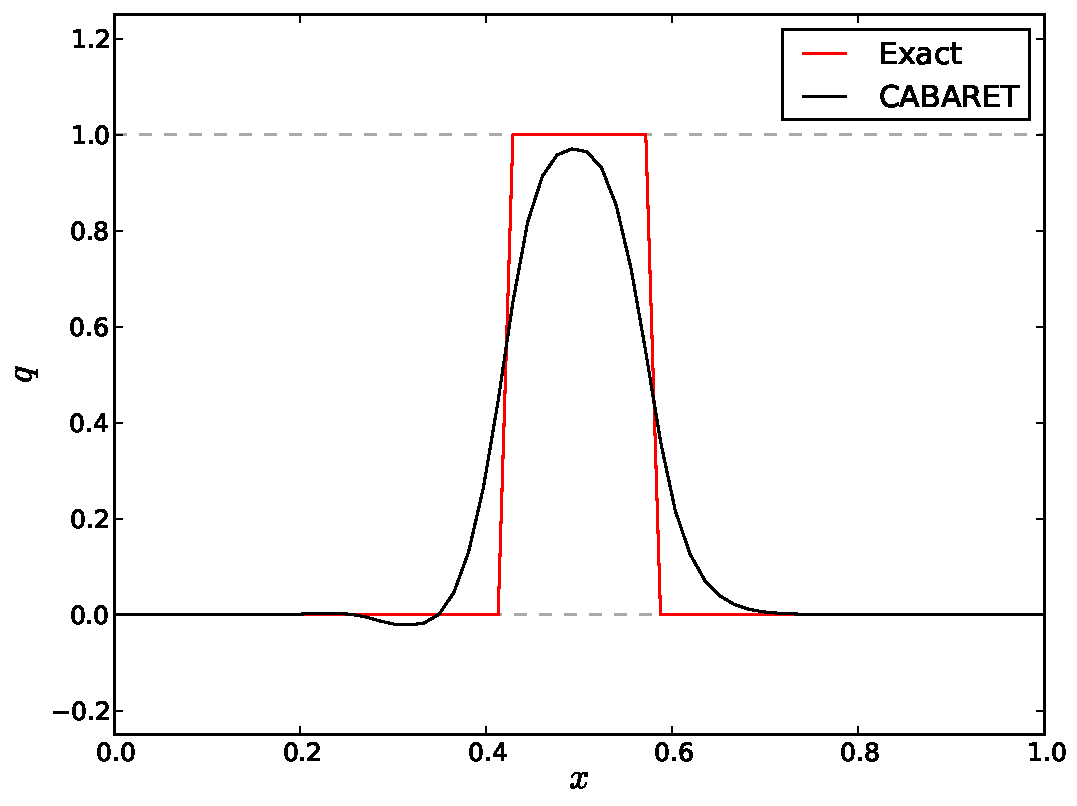
\includegraphics[width=0.45\textwidth]{figs/CabaretTopHat.pdf} &
        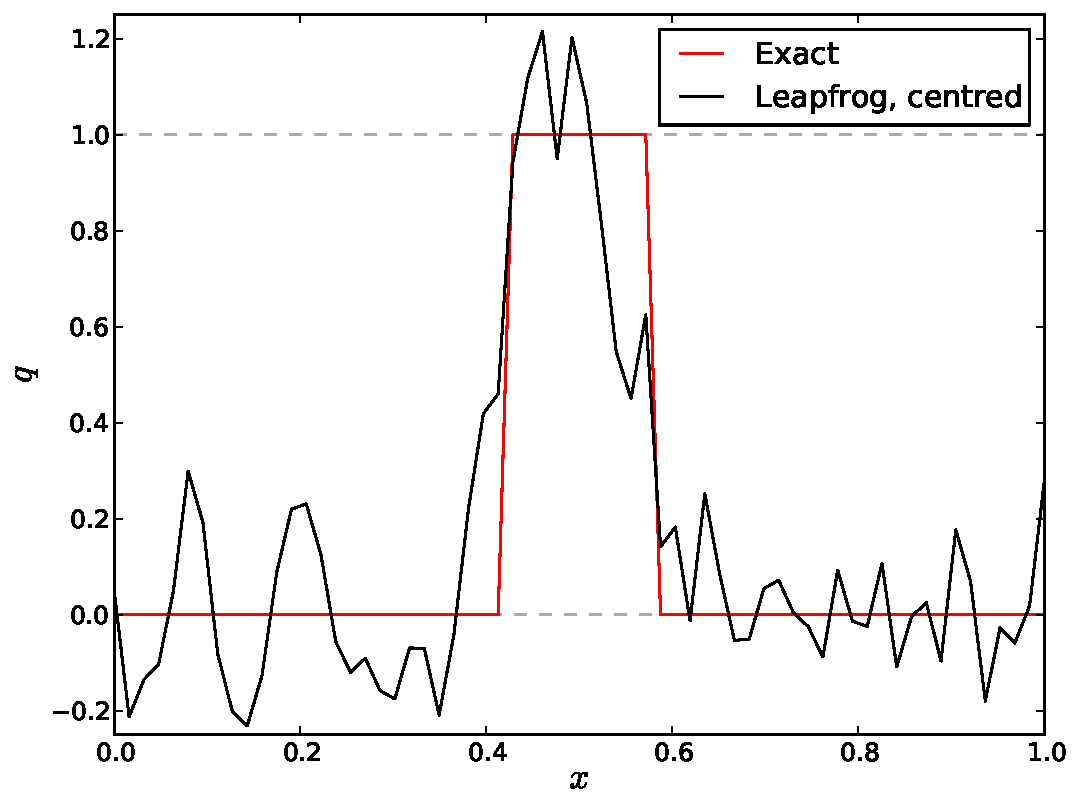
\includegraphics[width=0.45\textwidth]{figs/LeapfrogCentredTopHat.pdf} \\
      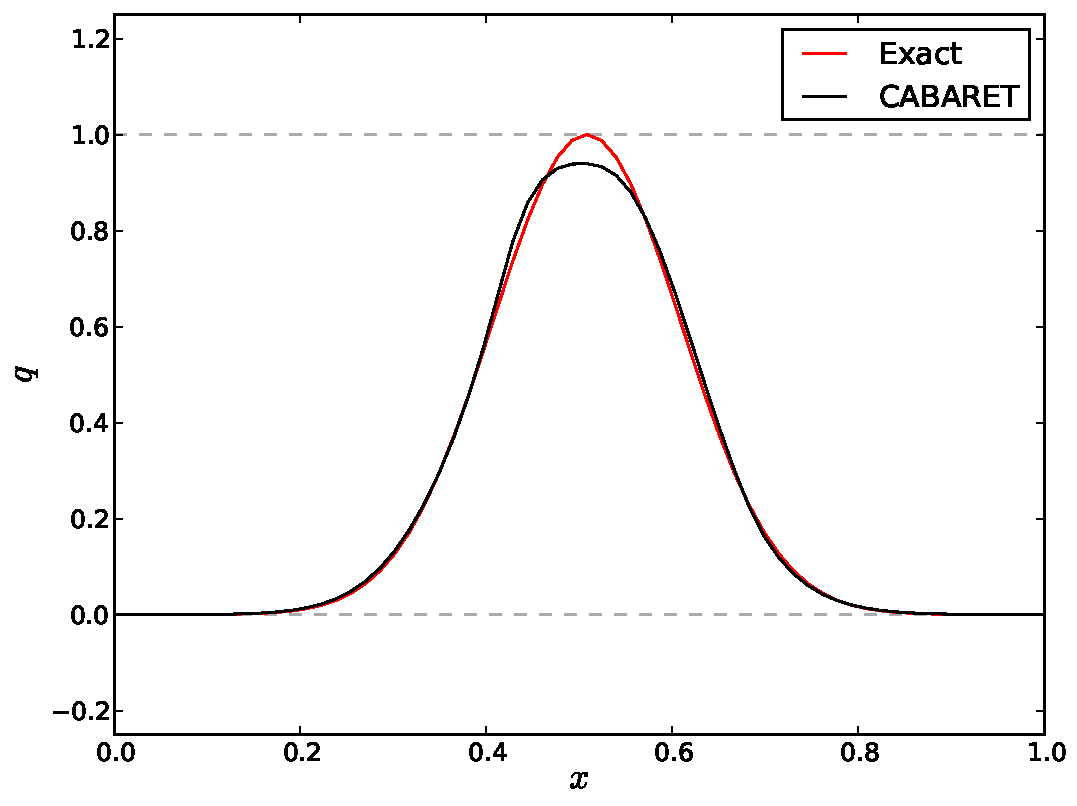
\includegraphics[width=0.45\textwidth]{figs/CabaretGaussian.pdf} &
        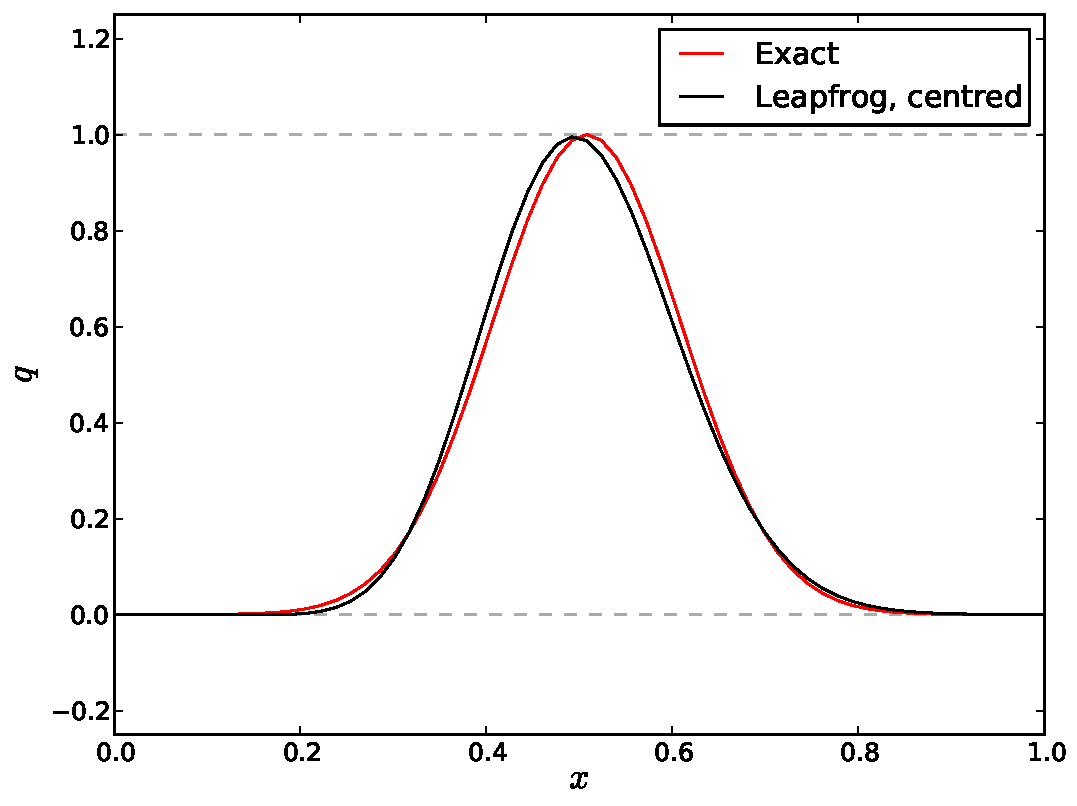
\includegraphics[width=0.45\textwidth]{figs/LeapfrogCentredGaussian.pdf}
    \end{tabular}
    \caption{One-dimensional advection by a constant velocity at Courant number $0.1$
             for one circuit of a periodic domain consisting of $64$ uniformly
             spaced grid points.
             Above: A top hat of width $10$ grid points.
             Below: A Gaussian with standard deviation $0.1$ times the domain
                    size.
             Left:  CABARET scheme.
             Right: Centred-in-space, centred-in-time (leapfrog) scheme (with no
                    time filter).}\label{fig:cabaret}
  \end{centering}
\end{figure}

\subsection{Advection of planetary vorticity}

The advection of planetary vorticity is treated using a second order scheme
of the form:
\begin{equation}
  \frac{q^{n + 1 / 2}_{i,j} - q^{n - 1 / 2}_{i,j}}{\Delta t} = -\frac{3}{2} \left[ \frac{1}{2} \left( v^n_{i,j + 1 / 2} + v^n_{i,j - 1 / 2} \right) \beta \right] - \frac{1}{2} \left[ \frac{1}{2} \left( v^{n - 1}_{i,j + 1 / 2} + v^{n - 1}_{i,j - 1 / 2} \right) \beta \right].
\end{equation}
See \citet{karabasov2009} for further details.

This has second order accuracy in space and time. Note that this conserves
the planetary vorticity (which follows as the velocity is divergence free).
Hence, since CABARET conserves the relative potential vorticity, the total
potential vorticity is also conserved \citep{karabasov2009}.

\subsection{Forcing and dissipation}

A time independent forcing, such as a time independent wind stress applied to
the upper layer, is discretised using forward Euler. This
leads to a tendency of:
\begin{equation}
  \frac{q^{n + 1 / 2}_{i,j} - q^{n - 1 / 2}_{i,j}}{\Delta t} = F_W.
\end{equation}

Diffusion is discretised using a backward scheme in time. This becomes, for the
fourth order diffusion tendency (see section \ref{sect:qgpv_forcing}):
\begin{equation}
  \frac{q^{n + 1 / 2}_{i,j} - q^{n - 1 / 2}_{i,j}}{\Delta t} = \frac{\nu}{\Delta x^2} \left[ \omega^{n + 1 / 2}_{i,j + 1} + \omega^{n + 1 / 2}_{i - 1,j} - 4 \omega^{n + 1 / 2}_{i,j} + \omega^{n + 1 / 2}_{i + 1,j} + \omega^{n + 1 / 2}_{i,j - 1} \right].
\end{equation}
The relative vorticity is computed using centred finite differencing:
\begin{equation}
  \omega^{n + 1 / 2}_{i,j} = \frac{1}{\Delta x^2} \left[ \psi^{n + 1 / 2}_{i,j + 1} + \psi^{n + 1 / 2}_{i - 1,j} - 4 \psi^{n + 1 / 2}_{i,j} + \psi^{n + 1 / 2}_{i + 1,j} + \psi^{n + 1 / 2}_{i,j - 1} \right],
\end{equation}
where the value of $\omega$ on the boundaries is determined as described in
section \ref{sect:cn_bc}. The resulting
discretisation of the fourth order diffusion term is second order
accurate in space.

Similarly, the tendency due to the second order bottom drag (see section
\ref{sect:qgpv_forcing}) is discretised via:
\begin{equation}
  \frac{q^{n + 1 / 2}_{i,j} - q^{n - 1 / 2}_{i,j}}{\Delta t} = -r \omega^{n + 1 / 2}_{i,j},
\end{equation}
with second order accuracy in space.

\subsection{Implementation details}\label{sect:cabaret_implementation}

\begin{enumerate}
  \item The relative potential vorticity $\zeta$ is used as the fundamental
        prognostic model variable.
  \item The values of the relative potential vorticity on the boundaries are
        computed from the stream function and relative vorticity, following
        application of the boundary condition for the relative vorticity.
  \item On the first timestep the terms associated with time level $n < 0$ are
        assigned a value of zero.
  \item The potential vorticity and stream function are collocated in time
        at time levels $n + 1 / 2$. Hence model diagnostics are computed
        at time levels $n + 1 / 2$.
  \item The CABARET implementation supports a time varying time step size. Following
        calculation of $u^n$ a new time step size, $\Delta t^{n + 1 / 2}$, is chosen
        such that:
        \begin{equation*}
          \frac{\left| \left| u^n \right| \right|_\infty \Delta t^{n + 1 / 2}}{\Delta x} = C,
        \end{equation*}
        where $C$ is
        a prescribed target Courant number. See \citet{karabasov2009} for a
        description of the modification of the time discretisation to support a
        varying time step size.
\end{enumerate}

\section{Potential vorticity inversion}\label{sect:pv_inversion}

This section describes the inversion of the potential vorticity $q$ to yield the
stream function $\psi$. In terms of vertical modes the inversion problem is as
per equation \eqref{eqn:zeta_modal}, i.e. for the $i$th mode:
\begin{equation}
   \left( \nabla^2 + l_i \right) \tilde{\psi}_i = \tilde{\zeta}_i = \tilde{q}_i - \beta y.
\end{equation}
This equation can be discretised in space using centred differencing for the
Laplace operator to yield:
\begin{equation}\label{eqn:zeta_modal_discrete}
  \tilde{\psi}_{i,j + 1,k} + \tilde{\psi}_{i - 1,j,k} + \left( l_k - 4 \right) \tilde{\psi}_{i,j,k} + \tilde{\psi}_{i + 1,j,k} + \tilde{\psi}_{i,j - 1,k} = \tilde{\zeta}_{i,j,k},
\end{equation}
where $X_{i,j,k}$ is the value of $X$ at node $i$ in the zonal direction,
$j$ in the meridional direction and for mode $k$, and
$2 \leq i \leq \left( N_i - 1 \right)$, $2 \leq j \leq \left( N_j - 1 \right)$.
This describes an implicit elliptic problem. Dirichlet boundary conditions are
required to close the system, and the boundary condition terms contribute to the
right-hand-side of the linear problem. The linear system can be written:
\begin{equation}
  \sum_{l = 1}^{N_i} \sum_{m = 1}^{N_j} L_{lmijk} \tilde{\psi}_{lmk} = \tilde{\zeta}_{ijk} - \tilde{g}_{ijk},
\end{equation}
or, more compactly:
\begin{equation}
  L_i \tilde{\psi}_i = \tilde{\zeta}_i - \tilde{g}_i,
\end{equation}
where $L_i$ is the discrete Helmholtz matrix and $-\tilde{g}_i$ are the
Dirichlet boundary condition contributions to the right-hand-side for each mode.

Given Dirichlet boundary conditions, the resulting linear elliptic problem is
inverted using a direct solver. A discrete sine transform is performed in the
meridional direction, yielding a series of sparse one-dimensional Helmholtz
problems in the zonal direction that can, for example, be inverted via Gaussian
elimination. An inverse discrete sine transform of the resulting solutions of
the one-dimensional problems completes the inversion. See \citet{hogg2006} for a complete
description of the method.

By the no-normal-flow boundary condition for $\uline{u}$ it follows that the
$\tilde{\psi}_i$ are equal to constants on each boundary:
\begin{equation}
  \tilde{\psi}_i = c_{ij} \quad \textrm{ on } \quad \partial \Omega_j,
\end{equation}
for each connected sub-surface $\partial \Omega_j$ of the domain $\Omega$. As stated the
$c_{ij}$ are not uniquely determined, and hence further constraints are required
in order to yield a unique set of $\tilde{\psi}_i$ and close the linear
problem \citep{mcwilliams1977}.

Section \ref{sect:simply_connected} details the
inversion problem in a simply connected domain, and section
\ref{sect:multiply_connected} details the inversion problem in a periodic
channel.

\subsection{Simply connected domain}\label{sect:simply_connected}

For a simply connected domain there is a single boundary constant per
mode. The value of the constant for the barotropic mode ($l_i = 0$) is arbitrary \linebreak
\citep{mcwilliams1977} and can be set to any constant.

An appropriate constraint for a simply connected domain is conservation of mass.
In the continuous case this implies that, at each $z$:
\begin{equation}
  \int_\Omega w_a = 0.
\end{equation}
By equation \eqref{eqn:qgpv_bc} this leads to, at each $z$:
\begin{equation}
  \partial_t \int_\Omega \psi = 0.
\end{equation}
Assuming that $\int_\Omega \psi = 0$ at some time (e.g. initially) this leads
to, in the layer model case:
\begin{equation}\label{eqn:mass_conservation}
  \int_\Omega \tilde{\psi}_i = 0,
\end{equation}
for all modes excluding the barotropic mode. For consistency, since the boundary
constant is arbitrary for the barotropic mode, this constraint can also be
applied for this mode.

Define $\tilde{\psi}^0_i$ and $\tilde{\psi}^1_i$ such that:
\begin{align}\label{eqn:simply_connected_decomposition}
  L_i \tilde{\psi}^0_i = \tilde{\zeta}_i, & & \tilde{\psi}^0 = 0 \quad \textrm{ on } \quad \partial \Omega, \nonumber \\
  L_i \tilde{\psi}^1_i = 1,               & & \tilde{\psi}^1 = 0 \quad \textrm{ on } \quad \partial \Omega,
\end{align}
Then:
\begin{equation}
  L_i \left( \tilde{\psi}^0_i + k_i \tilde{\psi}^1_i \right) = \tilde{\zeta}_i + k_i,
\end{equation}
which leads to:
\begin{equation}
  L_i \left[ \tilde{\psi}^0_i + k_i \left( \tilde{\psi}^1_i - \frac{1}{l_i} \right) \right] = \tilde{\zeta}_i.
\end{equation}
Hence we can write:
\begin{equation}
  \tilde{\psi}_i = \tilde{\psi}^0_i + k_i \left( \tilde{\psi}^1_i - \frac{1}{l_i} \right),
\end{equation}
and, since $\tilde{\psi}^0 = \tilde{\psi}^1 = 0$ on $\partial \Omega$:
\begin{equation}
  c_i = - \frac{k_i}{l_i}.
\end{equation}
By the integral constraint \eqref{eqn:mass_conservation}:
\begin{align}
  \int_\Omega \tilde{\psi}_i = 0 & \Rightarrow \int_\Omega \tilde{\psi}^0_i + k_i \left( \int_\Omega \tilde{\psi}^1_i - \frac{1}{l_i} \int_\Omega \right) = 0 \nonumber \\
                                & \Rightarrow k_i = - \frac{\int_\Omega \tilde{\psi}^0_i}{\int_\Omega \tilde{\psi}^1_i - \frac{1}{l_i} \int_\Omega} \nonumber \\
                                & \Rightarrow k_i = \frac{l_i \overline{\tilde{\psi}^0_i}}{1 - l_i \overline{\tilde{\psi}^1_i}}
\end{align}
where $\overline{\left( \ldots \right)}$ denotes ``domain-averaged''. Hence:
\begin{equation}\label{eqn:simply_connected_sf}
  \tilde{\psi}_i = \tilde{\psi}^0_i - \overline{\tilde{\psi}^0_i} \left( \frac{1 - l_i \tilde{\psi}^1_i}{1 - l_i \overline{\tilde{\psi}^1_i}} \right),
\end{equation}

Hence the potential vorticity inversion consists of two linear solves for
$\tilde{\psi}^0_i$ and $\tilde{\psi}^1_i$, as per equation
\eqref{eqn:simply_connected_decomposition}, together with the calculation of
$\tilde{\psi}_i$ as per equation \eqref{eqn:simply_connected_sf}. The solution
for the $\tilde{\psi}^1_i$ are performed once per simulation, and cached.

\subsection{Periodic channel}\label{sect:multiply_connected}

The mass conservation constraint is insufficient for the multiply connected
case. Additional constraints can be derived by imposing momentum conservation
constraints \citep{mcwilliams1977}. For details of the numerical implementation
of such constraints, see \citet{hogg2006}.

In \pequod, when using a periodic channel geometry, the following lateral
boundary conditions are used for the barotropic mode:
\begin{equation}
  \tilde{\psi}_1 \left( x, 0 \right) = \tilde{\psi}_1 \left( x, L_y \right),
\end{equation}
where the lateral boundaries are located at $y = 0$ and $y = L_y$. This boundary
condition imposes zero net barotropic shear. Since only one constraint is
required for the barotropic mode in this geometry \citep{mcwilliams1977}, one
can arbitrarily set:
\begin{equation}\label{eqn:bt_constraint}
  \tilde{\psi}_1 \left( x, 0 \right) = \tilde{\psi}_1 \left( x, L_y \right) = 0.
\end{equation}
The following boundary conditions are used for the baroclinic modes:
\begin{equation}\label{eqn:bc_constraint}
  \left. \int_{x = 0}^{L_x} \tilde{\zeta}_i dx \right|_{y = 0, L_y} = 0 \qquad i \geq 2,
\end{equation}
applied for the $\left( i - 1 \right)$th baroclinic mode, and where the domain has size $L_x$ in
the $x$-dimension. The discrete relative potential vorticity on the boundary can be written as
a function of the discrete stream function, via the partial-slip boundary
condition \eqref{eqn:discrete_partial_slip} or no-slip boundary condition
\eqref{eqn:discrete_no_slip}, and hence this yields constraints for the
$\tilde{\psi}_i$ ($i \geq 2$).

Note that this choice of boundary conditions does not yield momentum or mass
conservation. However, when combined with a background vertical shear as
discussed in section \ref{sect:shear}, the baroclinic boundary conditions
\eqref{eqn:bc_constraint} ensure that the vertical gradient of the background,
$x$-averaged, net horizontal potential vorticity gradient across the domain is not eroded by the dynamics.
Equivalently, the baroclinic boundary conditions can be considered a form of
lateral buoyancy forcing, which acts to maintain the vertical gradient of the background,
$x$-averaged, net horizontal potential vorticity gradient across the domain.

These boundary conditions are applied in the potential vorticity inversion in
the following manner. Define $\tilde{\psi}^0_i$, $\tilde{\psi}^1_i$, and
$\tilde{\psi}^2_i$, such that:
\begin{equation}\label{eqn:channel_decomposition}
  \tilde{\psi}_i = \tilde{\psi}^0_i + c_{i1} \tilde{\psi}^1_i + c_{i2} \tilde{\psi}^2_i,
\end{equation}
where:
\begin{align}
  L_i \tilde{\psi}^0_i = \tilde{\zeta}_i, & & \tilde{\psi}^0 = 0 \quad \textrm{ on } \quad \partial \Omega_S, & & \tilde{\psi}^0 = 0 \quad \textrm{ on } \quad \partial \Omega_N, \nonumber \\
  L_i \tilde{\psi}^1_i = 0,               & & \tilde{\psi}^1 = 0 \quad \textrm{ on } \quad \partial \Omega_S, & & \tilde{\psi}^1 = 1 \quad \textrm{ on } \quad \partial \Omega_N, \nonumber \\
  L_i \tilde{\psi}^2_i = 0,               & & \tilde{\psi}^2 = 1 \quad \textrm{ on } \quad \partial \Omega_S, & & \tilde{\psi}^2 = 0 \quad \textrm{ on } \quad \partial \Omega_N,
\end{align}
and where $\partial \Omega_S$ and $\partial \Omega_N$ are the southern and
northern boundaries respectively. For the barotropic mode $i = 0$ and, by
\eqref{eqn:bt_constraint}, $c_{11} = c_{12} = 0$. Define:
\begin{align}
  I_1 \left( \tilde{\psi}_i \right) = \left. \int_{x = 0}^{L_x} \tilde{\zeta}_i dx \right|_{y = 0}, \nonumber \\
  I_2 \left( \tilde{\psi}_i \right) = \left. \int_{x = 0}^{L_x} \tilde{\zeta}_i dx \right|_{y = L_y},
\end{align}
where the integrals on the right-hand-side are evaluated from the
$\tilde{\psi}_i$ via the partial-slip boundary condition \eqref{eqn:discrete_partial_slip}
or the no-slip boundary condition \eqref{eqn:discrete_no_slip}.
Then, since $I_1$ and $I_2$ are linear, and using the boundary condition
\eqref{eqn:bc_constraint}, for each baroclinic mode ($i \geq 2$):
\begin{align}
  c_{i1} I_1 \left( \tilde{\psi}^1_i \right) + c_{i2} I_1 \left( \tilde{\psi}^2_i \right) = - I_1 \left( \tilde{\psi}^0_i \right), \nonumber \\
  c_{i1} I_2 \left( \tilde{\psi}^1_i \right) + c_{i2} I_2 \left( \tilde{\psi}^2_i \right) = - I_2 \left( \tilde{\psi}^0_i \right).
\end{align}
This forms a $2 \times 2$ linear system for the $c_{ij}$,
$i \geq 2$.

Hence the potential vorticity inversion for the barotropic mode consists
of one linear solve for $\tilde{\psi}_1 = \tilde{\psi}^0_1$. The potential
vorticity inversion for each baroclinic mode consists of three linear solves for
$\tilde{\psi}^0_i$, $\tilde{\psi}^1_i$, and $\tilde{\psi}^2_i$, as per equation
\eqref{eqn:channel_decomposition}, together with the calculation of the
$c_{ij}$ via an inversion of a $2 \times 2$ linear system for the $c_{ij}$. The
solutions for the $\tilde{\psi}^1_i$, and $\tilde{\psi}^2_i$ are performed
once per simulation, and cached.

\chapter{Parallelisation}\label{sect:parallel}

This section provides a brief overview of the parallelisation method implemented
within \pequod.

The model is parallelised for distributed memory machines using MPI . A given
simulation is distributed across a given number of processes by designating a
sub-set of the model domain to each process. This defines the partitioning of
the problem, with each process assigned a partition of the global domain.

Section \ref{sect:qgpv_parallel} describes the parallelisation of the explicit
timestepping of the quasi-geostrophic potential vorticity equation
\eqref{eqn:qgpv_equation}. Section \ref{sect:pv_inversion_parallel} describes
the parallelisation of the implicit potential vorticity inversion step, defined
by equation \eqref{eqn:qgpv}. Details concerning the domain decomposition are
described in section \ref{sect:decomposition}.

\section{Quasi-geostrophic potential vorticity equation}\label{sect:qgpv_parallel}

The numerical solution of the quasi-geostrophic potential vorticity equation
\eqref{eqn:qgpv_equation}, using either the centred scheme or CABARET, involves
the solution of purely explicit problems -- no matrix inversion operations are
required (all left-hand-side matrices are the identity matrix). However,
differencing at partition boundaries requires information to be communicated
from adjacent processes.

This is achieved via the use of halo (or ghost) nodes. The local partition
assigned to each process is extended into neighbouring partitions, generating
an overlap region known as the ``halo''. The size of the halo (the number of
nodes in the overlap) is dependent upon the stencil of the discrete operator.
Information must be communicated periodically from processes ``owning'' the
nodes in the halo region (processes assigned the halo nodes in the original
partitioning) to all other processes which must access those nodes in
differencing.

\section{Potential vorticity inversion}\label{sect:pv_inversion_parallel}

The potential vorticity inversion step, defined by equation \eqref{eqn:qgpv} is
an implicit problem -- the Helmholtz problems must be inverted  in order to
obtain the stream function from the relative potential vorticity. Furthermore,
the ellipticity of the Helmholtz operator means that this is inherently a
non-local procedure -- information must be communicated from all nodes to all
other nodes, and hence from all processes to all other processes, in order to
perform the inversion.

This step is parallelised using a combination of data transposing and a
parallel solver for the one-dimensional Helmholtz problems. The system is
repartitioned (via communication) yielding a new partitioning that is contiguous
in the meridional direction (data transposing). This allows the discrete sine
transform in the meridional direction to be performed locally on each process.
The one-dimensional Helmholtz problems are inverted in parallel using the
\citet{schumann1995} algorithm. The inverse discrete sine transform step can be
performed locally. Finally, the system is repartitioned back to the original
partitioning.

\section{Domain decomposition}\label{sect:decomposition}

The potential vorticity inversion step involves a great deal of communication.
Hence it is advisable to choose a model partitioning that avoids the need
for repartitioning via data transposing. This is achieved by partitioning the
model only in the longitudinal direction.

\begin{figure}
  \begin{centering}
    \begin{tabular}{c}
      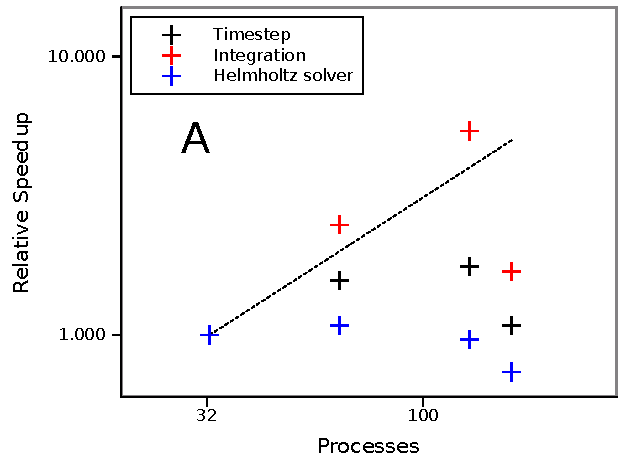
\includegraphics[width=0.6\textwidth]{figs/513x513x3_120327-scaling_speedup.pdf}
        \\
      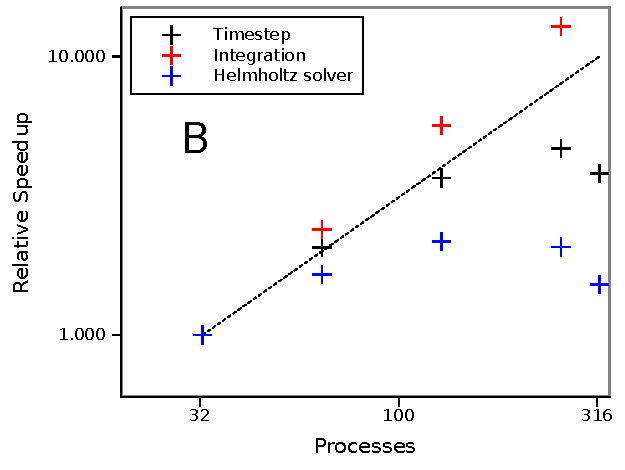
\includegraphics[width=0.6\textwidth]{figs/1025x1025x3_120327-scaling_speedup.pdf}
        \\
      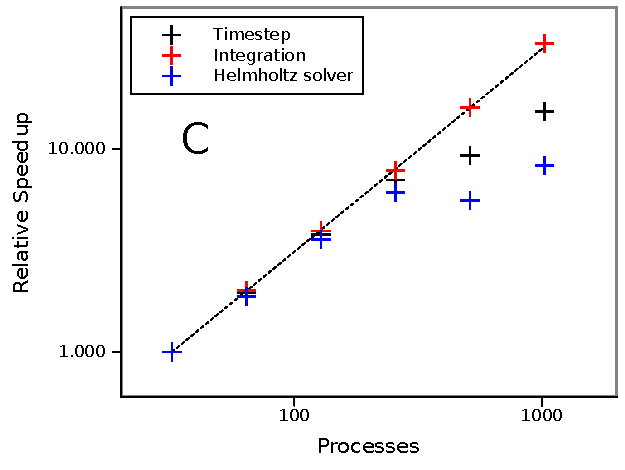
\includegraphics[width=0.6\textwidth]{figs/4097x4097x3_120327-scaling_speedup.pdf}
        \\
    \end{tabular}
    \caption{Relative parallel speedup of \pequod\ running with the CABARET
             scheme in a three-layer wind-driven square basin. All timings are
             recorded on the HECToR phase 3 using the performance diagnostics
             described in section \ref{sect:cost_diagnostics}. ``Timestep''
             refers to the total timestep runtime, ``Integration'' refers to the
             total time spent integrating the quasi-geostrophic potential
             vorticity equation, and ``Helmholtz'' refers to the total time
             spent performing the potential vorticity inversion. All timings
             exclude initialisation times. A: $513 \times 513$ grid. B:
             $1025 \times 1025$ grid. C: $4097 \times 4097$ grid.}\label{fig:speedup}
  \end{centering}
\end{figure}

Figure \ref{fig:speedup} shows the relative parallel speedup of \pequod\ on the
HECToR phase 3 for a three-layer wind driven square basin. These scaling tests
use a decomposition only in the longitudinal direction, and use the parallel
tri-diagonal solver of \citet{schumann1995}. The tests are performed using
\pequod\ version 0.9.3 and with \pequod\ compiled using the Cray Fortran
compiler version 8.0.1. Nodes on the HECToR phase 3 have $32$ cores, and the
tests shown use only fully populated nodes. The use of a single processor for
the $513 \times 513$ grid case has been found to be significantly more efficient
than the use of a fully populated node. This is possibly due to reduced data
contention, and could explain the super-linear speedup observed for the CABARET
integration with the $513 \times 513$ and $1025 \times 1025$ grids.

\chapter{Compiling the model}

This section describes how to compile \pequod. Section \ref{sect:dependencies}
describes model dependencies, section \ref{sect:make} describes compiler
options, and section \ref{sect:tests} describes model unit tests. Note that the
model must be recompiled each time the configuration files \verb+config.h+ or
\verb+qg3p_params.F90+ are modified (see section \ref{sect:configuration}).

\section{Dependencies}\label{sect:dependencies}

A small number of tools and libraries are required to compile \pequod. These are
typically available as part of a standard system, and hence you should not
normally need to compile them yourself. However, links to free and open source
versions are provided.

\subsection{Required dependencies}

The following are required for compilation of \pequod.

\subsubsection*{Make}

A standard tool used to assist in code compilation. GNU Make can be downloaded
from \url{http://www.gnu.org/software/make/}.

\subsubsection*{Fortran compiler}

\pequod\ in written primarily in Fortran 95, and makes use of a small number of
Fortran 2003 features. As such a fairly modern Fortran compiler is required.
\pequod\ has been compiled successfully with GCC version 4.6.3, and
with the Cray Fortran compiler version 8.0.4. GCC can be downloaded from
\url{http://gcc.gnu.org/}.

\subsubsection*{MPI}

An MPI implementation is required to compile and run the model. \pequod\
has been tested with Open MPI versions 1.4.3 and 1.6.1. Open MPI can be downloaded
from \url{http://www.open-mpi.org/}.

\subsubsection*{LAPACK}

LAPACK is a library of fundamental linear algebra routines. An implementation of
LAPACK is available from \url{http://www.netlib.org/lapack/}. Note that
optimised versions are usually available on clusters.

\subsection{Optional dependencies}\label{sect:optional_dependencies}

The following are optional. They may be used by model scripts or to build
documentation, or may be required when using experimental model features.

\subsubsection*{Python}

Python is used by several model scripts, including scripts used by the model
unit testing framework (see section \ref{sect:tests}). \pequod\ scripts have
been used successfully with Python version 2.7.3. Python can be
downloaded from \url{http://python.org/}.

\subsubsection*{NumPy}

Some model scripts make use of the Python NumPy module. NumPy can be downloaded
from \url{http://numpy.scipy.org/}. \pequod\ scripts have been used successfully
with NumPy version 1.6.1.

\subsubsection*{\LaTeX}

This manual is written in \LaTeX. Tex Live can be downloaded from
\url{http://www.tug.org/texlive/}.

\subsubsection*{PETSc}

PETSc is a library used to assist in the creation of numerical models, and is
required to compile \pequod\ when using the experimental \verb+PETSC+ option in
\verb+config.h+ (see section \ref{sect:config}). \pequod\ has been compiled
successfully with PETSc version 3.1. PETSc can be downloaded from
\url{http://www.mcs.anl.gov/petsc/}.

\section{Compilation}\label{sect:make}

\pequod\ is compiled via make. The file \verb+makefile.compiler+ can be used to
switch between compilers. For example:
\begin{lstlisting}[language = bash, frame = single]
include makefile.gfortran
\end{lstlisting}
selects the GNU fortran compiler, while:
\begin{lstlisting}[language = bash, frame = single]
include makefile.hector.cray
\end{lstlisting}
selects the Cray compiler for use on HECToR. Each compiler makefile defines a
series of variables that select the compiler and compiler flags. In particular,
the user may wish to modify:

\begin{longtable}{ | p{0.35\textwidth} | p{0.57\textwidth} | }
  \hline
  Macro & Description \\
  \hline
  \endhead
  \verb+INCLUDES+     & Options defining directories containing include files. \\
  \verb+LIBS+         & Options for linking against external libraries. \\
  \verb+DEBUG+        & Debugging build compiler flags. \\
  \verb+OPTIMISATION+ & Optimised build compiler flags. \\
  \hline
  \endfoot
\end{longtable}

In addition, the variable \verb+FCFLAGS+ defines options for the compilation of
free form Fortran files. While this should not generally be modified, each
compiler makefile contains two definitions for the variable, one with debugging
enabled and one with optimisation enabled. Commenting out the appropriate
version enables or disables debugging and optimisation. For example, in
\verb+makefile.gfortran+, debugging is enabled via:
\begin{lstlisting}[language = bash, frame = single]
#FCFLAGS = $(OPTIMISATION) $(FLAGS) \
  -ffree-line-length-none -DNDEBUG $(DEFINES) $(INCLUDES)
FCFLAGS = $(DEBUG) $(FLAGS) -ffree-line-length-none \
  -DDDEBUG $(DEFINES) $(INCLUDES)
\end{lstlisting}
while optimisation is enabled via:
\begin{lstlisting}[language = bash, frame = single]
FCFLAGS = $(OPTIMISATION) $(FLAGS) \
  -ffree-line-length-none -DNDEBUG $(DEFINES) $(INCLUDES)
#FCFLAGS = $(DEBUG) $(FLAGS) -ffree-line-length-none \
  -DDDEBUG $(DEFINES) $(INCLUDES)
\end{lstlisting}

Once a compiler makefile is selected and configured, the model is compiled via:
\begin{lstlisting}[language = bash, frame = single]
make qg3
\end{lstlisting}

Note that some compiler makefiles require the definition of the environment
variable \verb+MPI_DIR+. This should be set to the path of the local MPI
installation (typically \verb+/usr/+).

\section{Unit tests}\label{sect:tests}

\pequod\ contains a number of small test programs. These test only a very small
subset of model features. Hence the passing of these tests is a necessary, but
certainly not sufficient, requirement for correct model functionality. The exact
tests run depends upon the configuration as defined in \verb+config.h+ (see
section \ref{sect:config}).

The unit tests are compiled and run with the command:
\begin{lstlisting}[language = bash, frame = single]
make unittest
\end{lstlisting}

Note that the environment variable \verb+MPI_DIR+ must be defined in order to
execute the unit tests. This environment variable should be set to the path of
the local MPI installation (typically \verb+/usr/+).

\chapter{Model configuration}\label{sect:configuration}

This section describes the configuration of \pequod. The model is primarily
configured via compile-time options, defined in two files. \verb+config.h+
contains preprocessor definitions that enable and disable features within the
model. Options within this file are described in section \ref{sect:config}.
\verb+qg3p_params.F90+ contains all other compile-time model parameters, and is
described in section \ref{sect:qg3p_params}. Finally, section
\ref{sect:parameter_files} describes additional run-time parameter files that
may be specified.

The model must be recompiled each time either \verb+config.h+ or
\verb+qg3p_params.F90+ are modified (see section \ref{sect:make}).

\section{config.h}\label{sect:config}

\verb+config.h+ contains preprocessor definitions that enable and disable model
features. Options are enabled by defining a preprocessor macro, for example:
\begin{lstlisting}[language = C, frame = single]
#define WIND_FORCING
\end{lstlisting}
enables the option \verb+WIND_FORCING+, while:
\begin{lstlisting}[language = C, frame = single]
#undef WIND_FORCING
\end{lstlisting}
disables the option.

The following options enable and disable terms in the quasi-geostrophic
potential vorticity equation.

\begin{longtable}{ | p{0.35\textwidth} | p{0.57\textwidth} | }
  \hline
  Macro & Description \\
  \hline
  \endhead
  \verb+WIND_FORCING+      & Upper layer wind forcing. \\
  \verb+BACKGROUND_VSHEAR+ & Background vertical shear. \\
  \verb+BACKGROUND_HSHEAR+ & Background horizontal shear. \\

  \hline
  \endfoot
\end{longtable}

The following options enable and disable CABARET features.

\begin{longtable}{ | p{0.35\textwidth} | p{0.57\textwidth} | }
  \hline
  Macro & Description \\
  \hline
  \endhead
  \verb+CABARET+         & Enables the CABARET scheme. If disabled, the centred
                           scheme is used. \\
  \verb+CABARET_LIMITER+ & Enables the CABARET limiter. \\

  \hline
  \endfoot
\end{longtable}

The following options enable and disable features for the centred scheme. These
are primarily legacy options.

\begin{longtable}{ | p{0.35\textwidth} | p{0.57\textwidth} | }
  \hline
  Macro & Description \\
  \hline
  \endhead
  \verb+RA_DOUBLE_FILTER+        & Enables the Robert-Asselin-Williams time filter.
                                   If disabled, the standard Robert-Asselin filter
                                   is used. Recommended enabled. \\
  \verb+CENTRED_BOTTOM_FRICTION+ & If enabled, bottom friction is discretised
                                   using a centred scheme in time, rather than
                                   a forward scheme. Recommended disabled. \\
  \verb+FORWARD_EULER_START+     & If enabled, a forward Euler timestep is
                                   used for the first timestep. Otherwise the
                                   first timestep is initialised in an identical
                                   manner to the initial condition (i.e. zero
                                   valued or random valued relative potential
                                   vorticity). Recommended enabled. \\

  \hline
  \endfoot
\end{longtable}

The following options control the elliptic solver parallelisation. These are
advanced or experimental options that are used primarily for testing.

\begin{longtable}{ | p{0.35\textwidth} | p{0.57\textwidth} | }
  \hline
  Macro & Description \\
  \hline
  \endhead
  \verb+PH1D+         & Enables parallel solution of the 1D Helmholtz problems
                        using the \citet{schumann1995} algorithm. If disabled,
                        additional data transposing is performed and Gaussian
                        elimination is performed locally. \\
  \verb+PH1D_BUFFER+  & Buffers the global communications used by the
                        \citet{schumann1995} algorithm. \\
  \verb+INTERMEDIATE_TRANSPOSES+ & Transposes back to the original decomposition
                                   before and after the 1D Helmholtz solves.
                                   This greatly increases the amount of
                                   communication, but decreases the number of
                                   individual send / receives. Cannot be used
                                   with \verb+PH1D+. \\
  \verb+PETSC+        & Performs the potential vorticity inversion using PETSc. \\
  \verb+SUPERLU_DIST+ & Performs the potential vorticity inversion using the
                        SuperLU\_DIST parallel direct solver (via PETSc). \\

  \hline
  \endfoot
\end{longtable}

\section{qg3p\_params.F90}\label{sect:qg3p_params}

The majority of model options are set in the \verb+qg3p_params.F90+ Fortran
source file.

The following control the model grid and partitioning.

\begin{longtable}{ | p{0.35\textwidth} | p{0.57\textwidth} | }
  \hline
  Parameter & Description \\
  \hline
  \endhead
  \verb+layers+   & The number of model layers. \\
  \verb+iis+      & An array of meridional domain sizes, defining the
                    partitioning in the meridional direction. \\
  \verb+jjs+      & An array of zonal domain sizes, defining the partitioning in
                    the zonal direction. \\
  \verb+ii_m+     & The maximum value of \verb+iis+. Required for memory
                    allocation. \\
  \verb+jj_m+     & The maximum value of \verb+jjs+. Required for memory
                    allocation. \\
  \verb+periodic+ & Whether the domain is periodic in the zonal direction. \\
  \hline
  \endfoot
\end{longtable}

The parameters \verb+iis+, \verb+jjs+, \verb+ii_m+ and \verb+jj_m+ can be
generated using the \verb+qg_decomp+ script (see section \ref{sect:qg_decomp}).

The following control timestepping options.

\begin{longtable}{ | p{0.35\textwidth} | p{0.57\textwidth} | }
  \hline
  Parameter & Description \\
  \hline
  \endhead
  \verb+dt+              & The model timestep size, in $s$. If using adaptive
                           timestepping with CABARET, this is the size of the
                           first timestep. \\
  \verb+adapt_dt+        & Whether to use adaptive timestepping. Available only
                           with CABARET. \\
  \verb+max_dt+          & The maximum timestep size when using adaptive
                           timestepping, in $s$. Available only with CABARET. \\
  \verb+max_dt_increase+ & The maximum factor by which the timestep may increase
                           in each timestep adapt. Available only with
                           CABARET. \\
  \verb+target_cfl+      & The target Courant number when using adaptive
                           timestepping. Available only with CABARET. \\
  \verb+ra_nu+           & The Robert-Asselin filter strength ($\mu$ in equation
                           \eqref{eqn:modified_ra_filter}). Available only with
                           the centred scheme. \\
  \verb+ra_alpha+        & The Robert-Asselin-Williams filter parameter
                           ($\alpha$ in equation
                           \eqref{eqn:modified_ra_filter}). Available only with
                           the centred scheme. \\
  \verb+set_start_time+  & How to set the initial total model time. Has two
                           possible values: \verb+START_TIME_AUTO+ and
                           \verb+START_TIME_MANUAL+. \verb+START_TIME_AUTO+ sets
                           the initial total model time equal to zero or, if
                           \verb+start+ is set to \verb+START_PICKUP+, equal
                           to the total model time in input checkpoint files.
                           \verb+START_TIME_MANUAL+ allows one to override the
                           initial total model time, and set it equal to a
                           custom value. \\
  \verb+start_time_override+ & The initial total model time, in days, if
                               \verb+set_start_time+ is set to
                               \verb+START_TIME_MANUAL+. \\
  \verb+max_spin+        & Model spin-up time, in days. During this time model
                           time-average and eddy diagnostics are disabled. \\
  \verb+max_time+        & Run-time of the model after spin-up, in days. The
                           total model run-time is \verb+max_spin+ plus
                           \verb+max_time+. \\

  \hline
  \endfoot
\end{longtable}

The following control the physical parameters in the model. Note that wind
forcing in \pequod\ takes the form of:
\begin{align}\label{eqn:wind}
  F_{W,1} & = -\frac{\pi \tau_0}{L_y^* h_1} A_W \sin \frac{\pi \left( L_y^* + y^* \right)}{L_y^* + y_m}
                         & \textrm{ for } y^* \leq y_m, \\
          & = +\frac{\pi \tau_0}{L_y^* h_1} \frac{1}{A_W} \sin \left( \frac{\pi \left( y^* - y_m \right)}{L_y^* - y_m} \right)
                         & \textrm{ for } y^* > y_m,
\end{align}
where:
\begin{equation}\label{eqn:wind_shift}
  y_m = 2 C_W L_y^* + B_W x^* \frac{L_y^*}{L_x^*},
\end{equation}
and where $L_x^* = L_x / 2$, $L_y^* = L_y / 2$, $x^* = x - L_x^*$, and
$y^* = y - L_y^*$. $A_W$ can be used to generate an asymmetric wind stress,
$B_W$ can be used to tilt the wind stress with respect to the $x$-axis, and
$C_W$ can be used to offset the wind stress with respect to the domain centre.

\begin{longtable}{ | p{0.35\textwidth} | p{0.57\textwidth} | }
  \hline
  Parameter & Description \\
  \hline
  \endhead
  \verb+basinscale+ & The meridional extent of the model domain in cm. Internal
                      cells are square. Hence, combined with \verb+iis+ and
                      \verb+jjs+, this determines the horizontal dimensions of
                      the model domain. \\
  \verb+beta+       & Dimensional $\beta$ parameter, in
                      cm${}^{-1}$~s${}^{-1}$. \\
  \verb+set_strat+  & How to set the stratification. Has two possible values:
                      \verb+STRAT_RD+ and \verb+STRAT_INPUT+. \verb+STRAT_RD+
                      sets the stratification parameters using further
                      options in \verb+qg3p_params.F90+. \verb+STRAT_INPUT+
                      reads stratification parameters from a parameter file (see
                      section \ref{sect:stratification_input}). \\
  \verb+H+          & An array of layer thicknesses, in order of uppermost layer
                      to lowermost layer. Used only if \verb+set_strat+ is set
                      to \verb+STRAT_RD+. \\
  \verb+Rd_bcl1+    & First baroclinic deformation radius in cm. Used only if
                      \verb+set_strat+ is set to \verb+STRAT_RD+ and if there is
                      more than one layer. \\
  \verb+Rd_bcl2+    & Second baroclinic deformation radius in cm. Used only if
                      \verb+set_strat+ is set to \verb+STRAT_RD+ and if there
                      are more than two layers. \\
  \verb+tau+        & Wind stress magnitude strength per unit density, in
                      cm${}^2$~s${}^{-2}$ ($\tau_0$ in equation
                      \eqref{eqn:wind}). \\
  \verb+wind_shift+ & Parameter controlling the shift of the wind stress zero
                      line from the domain mid-latitude ($C_W$ in equation
                      \eqref{eqn:wind_shift}). \\
  \verb+wind_tilt+  & Parameter controlling the tilt of the wind stress zero
                      line relative to the zonal direction ($B_W$ in equation
                      \eqref{eqn:wind_shift}). \\
  \verb+wind_asym+  & Parameter controlling the asymmetry of the wind stress
                      to the North and South of the wind stress zero line ($A_W$
                      in equation \eqref{eqn:wind}). \\
  \verb+set_shear+  & How to set the background vertical shear. Has two possible
                      values: \verb+SHEAR_U+ and \verb+SHEAR_INPUT+.
                      \verb+SHEAR_U+ sets the shear using further options in
                      \verb+qg3p_params.F90+. \verb+SHEAR_INPUT+ reads shear
                      parameters from a parameter file (see section
                      \ref{sect:shear_input}). \\
  \verb+U+          & Background zonal velocity, setting the background vertical
                      shear, in cm~s${}^{-1}$. Used only if \verb+set_shear+ is
                      set to \verb+SHEAR_U+. \\
  \verb+u_background_h+ & Background zonal velocity function, setting the
                          background horizontal shear, in cm~s${}^{-1}$. The
                          argument \verb+y+ varies from zero at the south edge
                          of the domain to unity at the north edge of the
                          domain. \\
  \verb+visc+       & Laplacian viscosity coefficient, in
                      cm${}^2$~s${}^{-1}$. \\
  \verb+visc_bot+   & Bottom friction coefficient, in s${}^{-1}$. \\
  \hline
  \endfoot
\end{longtable}

The following control the model boundary conditions.

\begin{longtable}{ | p{0.35\textwidth} | p{0.57\textwidth} | }
  \hline
  Parameter & Description \\
  \hline
  \endhead
  \verb+partial_slip+ & Whether to use partial slip boundary conditions.
                        Otherwise no-slip boundary conditions are used. \\
  \verb+alpha+        & Partial slip length scale, in cm ($1 / \alpha$ in
                        equation \eqref{eqn:partial_slip}). Unused if
                        \verb+partial_slip+ is set to \verb+.false.+ . \\
  \hline
  \endfoot
\end{longtable}

Finally, the following control model initialisation and output.

\begin{longtable}{ | p{0.35\textwidth} | p{0.57\textwidth} | }
  \hline
  Parameter & Description \\
  \hline
  \endhead
  \verb+k_out+  & Time, in days, between output of diagnostics. \\
  \verb+k_save+ & Time, in days, between output of model output files. \\
  \verb+k_dump+ & Number of outputs written before a new model output file is
                  created. \\
  \verb+k_cp+   & Number of outputs written before a full model checkpoint is
                  written. Applies only when using CABARET. \\
  \verb+quad+   & Whether to compute and output model eddy diagnostics. \\
  \verb+start+  & How to start the model. Has three possible values:
                  \verb+START_ZERO+, \verb+START_PERTURB+, and
                  \verb+START_PICKUP+. \verb+START_ZERO+ initialises the model
                  with zero relative potential vorticity and stream function.
                  \verb+START_PERTURB+ starts the model with a random interior
                  relative potential vorticity field. \verb+START_PICKUP+
                  initialises the model from a checkpoint (see section
                  \ref{sect:checkpoint_files}).\\
  \verb+zeta_perturb+ & Maximum magnitude of perturbations of the relative
                        potential vorticity when \verb+start+ is set to
                        \verb+START_PERTURB+, in units of s${}^{-1}$. \\
  \verb+save_log+     & If enabled, writes standard output and standard error
                        to log files. \\
  \hline
  \endfoot
\end{longtable}

\section{Supplementary parameter files}\label{sect:parameter_files}

In addition to \verb+config.h+ and \verb+qg3p_params.F90+, a number of
supplementary parameter files may be used to configure the model. The use of
these parameter files is optional, and is dependent upon options defined in
\verb+qg3p_params.F90+.

\subsection{Stratification parameters}\label{sect:stratification_input}

If \verb+set_strat+ is set to \verb+STRAT_INPUT+ in \verb+qg3p_params.F90+ (see
section \ref{sect:qg3p_params}) then stratification parameters are read from
a parameter file located in \linebreak \verb+./input/stratification+ relative
to the program working directory. Note that such a parameter file must be
specified if using more than three model layers.

The stratification parameter file is a plain text file defining the layer
thicknesses, and the stratification parameters $s_i^-$ and $s_i^+$ defined
in equation \eqref{eqn:stratification_parameters}. The first line of the
file is a single integer defining the number of layers. All remaining lines
contain up to three floating point numbers, defining the stratification
parameters in order of uppermost to lowermost layer. For each line the
floating point numbers define, in order: the layer thickness $h_i$, the
stratification parameter $s_i^-$, and the stratification parameter $s_i^+$.
Note that $s_i^-$ is not defined for the first layer, and $s_i^+$ is not defined
for the last layer. The $h_i$ are in units of cm, and the $s_i^-$ and $s_i^+$
are in units of cm~$^{-2}$.

The following is an example of a three layer stratification parameter file:
\begin{lstlisting}[language = sh, frame = single]
3
0.25E+5 0.11861888862549392E-12
0.75E+5 0.39539629541831307E-13 0.74701918925497074E-13
0.30E+6 0.18675479731374269E-13
\end{lstlisting}
This defines three layers with upper layer thickness $250$~m, middle layer
thickness $750$~m and lower layer thickness $3000$~m. The stratification
parameters defined correspond to a first baroclinic deformation radius of
$40$~km and a second baroclinic deformation radius of $23$~km.

\subsection{Shear parameters}\label{sect:shear_input}

If \verb+set_shear+ is set to \verb+SHEAR_INPUT+ in \verb+qg3p_params.F90+ (see
section \ref{sect:qg3p_params}) then vertical shear parameters are read from
a parameter file located in \linebreak \verb+./input/u+ relative
to the program working directory.

The shear parameter file is a plain text file defining the background zonal
velocity. The first line of the
file is a single integer defining the number of layers. All remaining lines
contain one floating point number, defining the background zonal
velocity in order of uppermost to lowermost layer. The velocities are defined
in units of cm~s${}^{-1}$.

The following is an example of a three layer shear parameter file:
\begin{lstlisting}[language = sh, frame = single]
3
6.0
3.0
0.0
\end{lstlisting}
This defines a background zonal velocity of 6~cm~s${}^{-1}$ in the upper layer,
3~cm~s${}^{-1}$ in the middle layer, and zero in the lower layer.

\subsection{Checkpoint files}\label{sect:checkpoint_files}

If \verb+start+ is set to \verb+START_PICKUP+ in \verb+qg3p_params.F90+ (see
section \ref{sect:qg3p_params}) then the model is initialised using checkpoint
files located in \verb+./input+ relative to the program working directory.
The checkpoint files are formatted as per normal model output, but with the
output file number neglected. Note that, when using CABARET, supplementary
data files are also required. The frequency of output of supplementary data
files is controlled by the \verb+k_cp+ parameter in \verb+qg3p_params.F90+ (see
section \ref{sect:qg3p_params}).

Checkpoint files can be copied into \verb+./input+ using the \verb+qg_pickup+
script (see section \ref{sect:qg_pickup}).

\chapter{Model output and diagnostics}

This chapter details the \pequod\ model output data and online diagnostics. The
formatting and types of model output data are described in section
\ref{sect:output}. Additional diagnostics output to standard output (or to
log files if the \verb+log_output+ option is enabled -- see section
\ref{sect:qg3p_params}) are described in section \ref{sect:log_output}.

\section{Model output}\label{sect:output}

This section describes \pequod\ model output, excluding data output to standard
output (or model log files if the \verb+log_output+ option is enabled in
\linebreak \verb+qg3p_params.F90+ -- see section \ref{sect:qg3p_params}).
Model array indexing and \linebreak non-dimensionalisation are detailed in
sections \ref{sect:indexing} and \ref{sect:non_dimensionalisation} respectively.
The output file format is detailed in section \ref{sect:output_format}, and the
data output by the model in this format is listed in section
\ref{sect:output_files}.

\subsection{Array indexing}\label{sect:indexing}

\pequod\ uses array style indexing for model variables. That is, the
latitudinal index \verb+i+ refers to the \verb+i+~th row of nodes counting
southward from the north edge of the domain, the longitudinal index \verb+j+
refers to the \verb+j+~th column of nodes counting eastward from the west edge
of the domain, the latitudinal domain size \verb+ii+ refers to the total number
of nodes in the latitudinal direction, and the longitudinal domain size
\verb+jj+ refers to the total number of nodes in the longitudinal
direction\footnote{The \emph{only} exception to this convention is the indexing
of the partitioning in the meta-data files, \texttt{p\_i}, \texttt{p\_j},
\texttt{p\_ii}, and \texttt{p\_jj} described in section
\ref{sect:output_format}}.

\subsection{Non-dimensionalisation}\label{sect:non_dimensionalisation}

Most model data is non-dimensionalised. For a model variable with dimensions
$L^a T^b$, where $L$ is a length scale and $T$ a time scale, to convert to cgs
units one multiplies by \verb+l_scale+${}^a$~\verb+t_scale+${}^b$.
\verb+l_scale+ and \verb+t_scale+ are output to meta-data files, as described in
section \ref{sect:output_format}.

\subsection{Output file format}\label{sect:output_format}

This section describes the file format used to store output model data.
For a given data set each process outputs two files: a plain text file
containing meta-data, and a binary file containing the output data itself.

The meta-data file has name:
\begin{lstlisting}[language = bash, frame = single]
base[.process]
\end{lstlisting}
where \verb+base+ is a filename prefix common to a given data set and
\verb+process+ is the process number (indexed from zero). The process number is
absent for serial simulations. The following is output at the start of the
meta-data file, in plain text.
\begin{lstlisting}[language = bash, frame = single]
        n    p_ii    p_jj       p     p_i     p_j
     g_ii    g_jj  layers
     ii_0    jj_0      ii      jj
  l_scale t_scale
\end{lstlisting}
where the variables have the following values:
\begin{longtable}{ | p{0.21\textwidth} | p{0.12\textwidth} | p{0.57\textwidth} | }
  \hline
  Variable & Type & Value \\
  \hline
  \endhead
  \verb+n+       & integer & The total number of processes. \\
  \verb+p_ii+    & integer & The decomposition size in the longitudinal
                             direction (the size of \verb+jjs+ in
                             \verb+qg3p_params.F90+ - see section
                             \ref{sect:qg3p_params}). \\
  \verb+p_jj+    & integer & The decomposition size in the latitudinal direction
                             (the size of \verb+iis+ in \verb+qg3p_params.F90+ -
                             see section \ref{sect:qg3p_params}). \\
  \verb+p+       & integer & The process number, indexed from zero. \\
  \verb+p_i+     & integer & The longitudinal position of the process in the
                             domain partitioning, counting eastward from the
                             west edge of the domain and indexed from one. \\
  \verb+p_j+     & integer & The latitudinal position of the process in the
                             domain partitioning, counting northward from the
                             south edge of the domain and indexed from one. \\
  \verb+g_ii+    & integer & The global domain size in the latitudinal
                             direction. \\
  \verb+g_jj+    & integer & The global domain size in the longitudinal
                             direction. \\
  \verb+layers+  & integer & The number of model layers. \\
  \verb+ii_0+    & integer & The index of the upper row of the local process
                             array in the global array, counting southward from
                             the north edge of the domain and indexed from zero. \\
  \verb+jj_0+    & integer & The index of the left column of the local process
                             array in the global array, counting eastward from
                             the west edge of the domain and indexed from zero. \\
  \verb+ii+      & integer & The local domain size in the latitudinal direction. \\
  \verb+jj+      & integer & The local domain size in the longitudinal
                             direction. \\
  \verb+l_scale+ & double precision & Space normalisation factor. \\
  \verb+t_scale+ & double precision & Time normalisation factor. \\
  \hline
  \endfoot
\end{longtable}
The remainder of the meta-data file consists of a list of variable names and
variable shapes. The possible sizes for each variable index are:
\begin{longtable}{ | p{0.35\textwidth} | p{0.57\textwidth} | }
  \hline
  Variable size & Value \\
  \hline
  \endhead
  \verb+ii+         & The local domain size in the latitudinal direction. \\
  \verb+jj+         & The local domain size in the longitudinal direction. \\
  \verb+layer+      & The number of model layers. \\
  \verb+interface+  & The number of model interfaces (the number of layers minus
                      one). \\
  \verb+leapfrog+   & The number of timesteps stored by the model when
                      leapfrogging (always equal to two). \\
  \verb+flux_i_ii+  & The local domain size in the latitudinal direction for
                      an array staggered in the longitudinal direction. \\
  \verb+flux_i_jj+  & The local domain size in the longitudinal direction for
                      an array staggered in the longitudinal direction. \\
  \verb+flux_j_ii+  & The local domain size in the latitudinal direction for
                      an array staggered in the latitudinal direction. \\
  \verb+flux_j_jj+  & The local domain size in the longitudinal direction for
                      an array staggered in the latitudinal direction. \\
  \hline
  \endfoot
\end{longtable}
The following is an example of a meta-data file for time-averaged model data:
\begin{lstlisting}[language = bash, frame = single]
      24      24       1       0       1       1
     513     513       3
       0       0     513      21
  0.75e6  0.75e6
model_time_day
total_time_day
psi1_av  ii jj
psi2_av  ii jj
psi3_av  ii jj
\end{lstlisting}
This describes output for process $0$ of a $24$ process simulation decomposed
only in the longitudinal direction, with two scalar variables
\verb+model_time_day+ and \verb+total_time_day+, and three variables each
defined for a single model layer.

The binary data file has name:
\begin{lstlisting}[language = bash, frame = single]
base.d[.process]
\end{lstlisting}
where \verb+base+ is a filename prefix common to a given data set and
\verb+process+ is the process number (indexed from zero). The process number is
absent for serial simulations. Each variable listed in the meta-data file is
output, in order, to the binary data file in the form:
\begin{lstlisting}[language = bash, frame = single]
[header][data][footer]
\end{lstlisting}
\verb+header+ consists of a default Fortran integer listing the number of bytes
stored in \verb+data+. \verb+data+ is a binary array of eight byte double
precision values. \verb+footer+ is a further default Fortran integer, again
equal to the number of bytes stored in \verb+data+. This formatting is
consistent with Fortran unformatted binary output on most platforms. Arrays are
output using column-major ordering. Model variables are output with array style
indexing, with the latitudinal index \verb+i+ counting southward from the north
edge of the domain and the longitudinal index \verb+j+ counting eastward from
the west edge of the domain (see section \ref{sect:indexing}).

\subsection{Output files}\label{sect:output_files}

There are three types of data output in format described in the previous
section: snapshot data, time-averaged data, and eddy diagnostics.

\subsubsection{Snapshot data files}\label{sect:snapshot_data_files}

Snapshot data files have filename \verb+base+:
\begin{lstlisting}[language = bash, frame = single]
qg[layers]_[ii]_s.[index]
\end{lstlisting}
where \verb+layers+ is the number of model layers, \verb+ii+ is the model
domain size in the latitudinal direction, and \verb+index+ is an integer.
\verb+index+ counts from zero, and is incremented after every
\verb+k_out+~$\times$~\verb+k_save+ days, where \verb+k_out+ and \verb+k_save+
are defined in \verb+qg3p_params.F90+ (see section \ref{sect:qg3p_params}).

When using the centred scheme snapshot data files contain the following
variables with the indicated shapes (as defined in meta-data files -- see
section \ref{sect:output_format}):
\begin{lstlisting}[language = bash, frame = single]
model_time_day
total_time_day
psi1            ii  jj  leapfrog
...
psi[layers]     ii  jj  leapfrog
zeta1           ii  jj  leapfrog
...
zeta[layers]    ii  jj  leapfrog
\end{lstlisting}
When using the CABARET scheme snapshot data files contain the following
variables with the indicated shapes:
\begin{lstlisting}[language = bash, frame = single]
model_time_day
total_time_day
psi1            ii  jj
...
psi[layers]     ii  jj
zeta1           ii  jj
...
zeta[layers]    ii  jj
\end{lstlisting}

\verb+model_time_day+ is the time, in days, executed by the current instance of
the model. When picking up a simulation from checkpoint data using the
\verb+START_PICKUP+ option in \verb+qg3p_params.F90+ (see section
\ref{sect:qg3p_params}) this variable returns to a value of zero.
\verb+total_time_day+ is the total simulation time, in days. When picking up a
simulation from checkpoint data using the \verb+START_PICKUP+ option in
\verb+qg3p_params.F90+ the value of this variable is preserved. \verb+psi[N]+ is
the stream function and \verb+zeta[N]+ is the relative potential vorticity,
each defined for layer $N$. The \verb+psi[N]+ and \verb+zeta[N]+ are output in
non-dimensional units (see section \ref{sect:non_dimensionalisation}).

When using the centred scheme the \verb+psi[N]+ and \verb+zeta[N]+ are output
at two time levels: the current model time level $n$ and the previous time
level $n - 1$. This is indicated by the \verb+leapfrog+ index size. Using
Fortran array indexing, \verb+psi(:, :, 1)+ contains data from time level
$n - 1$ and \verb+psi(:, :, 2)+ contains data from time level $n$ (the time
indicated by \verb+model_time_day+ and \verb+total_time_day+).

\subsubsection{Time-averaged data files}

Time-averaged data files have filename \verb+base+:
\begin{lstlisting}[language = bash, frame = single]
qg[layers]_[ii]_s_av
\end{lstlisting}
where \verb+layers+ is the number of model layers and \verb+ii+ is the model
domain size in the latitudinal direction.

Time-averaged data files contain the time-averages of fields. The time-averages
are taken only after the time indicated by the \verb+max_spin+ parameter in
\verb+qg3p_params.F90+ (see section \ref{sect:qg3p_params}). Time-averaged
data files contain the following variables (as defined in meta-data files -- see
section \ref{sect:output_format}):
\begin{lstlisting}[language = bash, frame = single]
model_time_day
total_time_day
psi1_av         ii  jj
...
psi[layers]_av  ii  jj
\end{lstlisting}

\verb+model_time_day+ and \verb+total_time_day+ are defined as for snapshot
data files. \verb+psi[N]_av+ is the time-averaged stream function in the $N$th
model layer, in non-dimensional units (see section
\ref{sect:non_dimensionalisation}).

\subsubsection{Eddy diagnostic data files}

Eddy diagnostic data files have filename \verb+base+:
\begin{lstlisting}[language = bash, frame = single]
qg[layers]_[ii]_quad_av
\end{lstlisting}
where \verb+layers+ is the number of model layers and \verb+ii+ is the model
domain size in the latitudinal direction.

Eddy diagnostic data files contain the time-averages of products of fields. The
time-averages are only taken only after the time indicated by the
\verb+max_spin+ parameter in \verb+qg3p_params.F90+ (see section
\ref{sect:qg3p_params}). Combined with data from the time-averaged data files,
these data enable eddy covariances to be computed. Eddy diagnostic data files
contain the following variables (as defined in meta-data files -- see section
\ref{sect:output_format}):
\begin{lstlisting}[language = bash, frame = single]
model_time_day
total_time_day
uu_av           ii  jj  layer
vv_av           ii  jj  layer
uu_i_av         ii  jj  interface
vv_i_av         ii  jj  interface
uv_av           ii  jj  layer
ur_av           ii  jj  layer
vr_av           ii  jj  layer
rr_av           ii  jj  layer
pr_av           ii  jj  layer
uz_av           ii  jj  layer
vz_av           ii  jj  layer
zz_av           ii  jj  layer
zr_av           ii  jj  layer
pp_av           ii  jj  layer
pz_av           ii  jj  layer
sc_ub_av        ii  jj  interface
sc_vb_av        ii  jj  interface
sc_bb_av        ii  jj  layer
sc_bb_i_av      ii  jj  interface
\end{lstlisting}

\verb+model_time_day+ and \verb+total_time_day+ are defined as for snapshot
data files. The values of the remaining variables are listed below.
\begin{longtable}{ | p{0.25\textwidth} | p{0.67\textwidth} | }
  \hline
  Diagnostic & Value \\
  \hline
  \endhead
  \verb+uu_av+      & $\overline{u^2}$ on layers. \\
  \verb+vv_av+      & $\overline{v^2}$ on layers. \\
  \verb+uu_i_av+    & $\overline{u^2}$ on interfaces. \\
  \verb+vv_i_av+    & $\overline{v^2}$ on interfaces. \\
  \verb+ur_av+      & $\overline{u \omega}$ on layers. \\
  \verb+vr_av+      & $\overline{v \omega}$ on layers. \\
  \verb+rr_av+      & $\overline{\omega^2}$ on layers. \\
  \verb+pr_av+      & $\overline{\psi \omega}$ on layers. \\
  \verb+uz_av+      & $\overline{u \zeta}$ on layers. \\
  \verb+vz_av+      & $\overline{v \zeta}$ on layers. \\
  \verb+zz_av+      & $\overline{\zeta^2}$ on layers. \\
  \verb+pp_av+      & $\overline{\psi^2}$ on layers. \\
  \verb+pz_av+      & $\overline{\psi \zeta}$ on layers. \\
  \verb+sc_ub_av+   & The layer model discretisation of
                      $\frac{f_0}{N_0^2} \overline{u b}$, equal to
                      $\frac{1}{2} h_i s_i^+ \overline{\left( u_i + u_{i + 1} \right) \left( \psi_i - \psi_{i + 1} \right)}$
                      for each interface $i$. \\
  \verb+sc_vb_av+   & The layer model discretisation of
                      $\frac{f_0}{N_0^2} \overline{v b}$, equal to
                      $\frac{1}{2} h_i s_i^+ \overline{\left( v_i + v_{i + 1} \right) \left( \psi_i - \psi_{i + 1} \right)}$
                      for each interface $i$. \\
  \verb+sc_bb_av+   & The layer model discretisation of
                      $\frac{1}{2 N_0^2} \overline{bb}$ on layers, equal to
                      $\frac{1}{4} \left[ s_i^- \overline{\left( \psi_{i - 1} - \psi_i \right)^2} + s_i^+ \overline{\left( \psi_i - \psi_{i + 1} \right)^2} \right]$
                      for each layer $i$, where the $s_i^-$ term is omitted for
                      the uppermost layer and the $s_i^+$ term is omitted for
                      the lowermost layer. \\
  \verb+sc_bb_i_av+ & The layer model discretisation of
                      $\frac{1}{2 N_0^2} \overline{bb}$ on interfaces, equal to
                      $\frac{h_i s_i^+}{h_i + h_{i + 1}} \overline{\left( \psi_i - \psi_{i + 1} \right)^2}$
                      for each interface $i$. \\
  \hline
  \endfoot
\end{longtable}
The velocity components on layers are computed via centred differencing, and the
velocity components on interfaces are computed via averaging of the values on
adjacent layers.

\section{Additional diagnostics}\label{sect:log_output}

This section describes model diagnostics that are output to standard output,
or to model log files if the \verb+log_output+ option is enabled. The frequency
of diagnostic output is controlled by the \verb+k_out+ option (see section
\ref{sect:qg3p_params}).

These diagnostics always output the current model time, in units of days and
units of years ($365$ days). When running with the CABARET scheme the model
timestep size is also output, in units of seconds and units of hours. Energy
and performance diagnostics are then output. Energy diagnostics are described in
section \ref{sect:energy_diagnostics} and performance diagnostics are described
in section \ref{sect:cost_diagnostics}.

\subsection{Energy diagnostics}\label{sect:energy_diagnostics}

The energy diagnostics record the layer kinetic energies and the total model
potential energy.

The discrete layer integrated kinetic energy density for layer $k$ is given by:
\begin{align}
  K_k = \sum_{i=2}^{N_i} \sum_{j = 2}^{N_j} \frac{h_k}{8}
                        \left[ \left( \psi_{i,j - 1,k} - \psi_{i - 1,j - 1,k} + \psi_{i,j,k} - \psi_{i - 1,j,k} \right)^2 \right. \\
    \quad \quad \quad + \left. \left( \psi_{i - 1,j,k} - \psi_ {i - 1,j - 1,k} + \psi_{i,j,k} - \psi_{i,j - 1,k} \right)^2 \right].
\end{align}
The model outputs $K_k / \left( L_x L_y H \right)$ in non-dimensional units (see
section \ref{sect:non_dimensionalisation}). The discrete interface integrated
potential energy density for interface $k$ is given by:
\begin{equation}
  P_k = \sum_{i=1}^{N_i} \sum_{j=1}^{N_j} \frac{a_{i,j} h_k s_k^+}{2} \left( \psi_{i,j,k} - \psi_{i,j,k + 1} \right)^2,
\end{equation}
where $a_{i,j}$ equals one for interior nodes, one quarter for corner nodes, and
one half for other boundary nodes. The model outputs
$\sum_k P_k / \left( L_x L_y H\right)$ in non-dimensional units (see section
\ref{sect:non_dimensionalisation}).

\subsection{Performance diagnostics}\label{sect:cost_diagnostics}

The performance diagnostics record the time taken by the model in executing
various sections of the code. The diagnostics are measured by the
\verb+mpi_wtime+ MPI subroutine, called by the first process and excluding all
initialisation times. The times reported are in units of seconds, and are given
together with a percentage of the total timestep loop runtime (rounding down).

The following diagnostics are recorded when running in serial or parallel:
\begin{longtable}{ | p{0.35\textwidth} | p{0.57\textwidth} | }
  \hline
  Diagnostic & Value \\
  \hline
  \endhead
  Total       & The total time spent executing the main timestep loop. \\
  Integration & The time spent integrating the quasi-geostrophic potential
                vorticity equation using either the centred scheme or the
                CABARET scheme. \\
  Helmholtz   & The time spent performing the potential vorticity inversion. \\
  Diagnostics & The time spent computing time-averaged and eddy diagnostics. \\
  Other       & All other model costs. This includes model output. \\
  \hline
  \endfoot
\end{longtable}
When running in parallel additional performance diagnostics recording the cost
of communication are output. The exact parallel performance diagnostics are
dependent upon options defined in \verb+config.h+ (see section
\ref{sect:config}).
\begin{longtable}{ | p{0.35\textwidth} | p{0.57\textwidth} | }
  \hline
  Diagnostic & Value \\
  \hline
  \endhead
  Transpose         & The time spent, by the first process, waiting for
                      transpose communications to complete for the parallel
                      Helmholtz solver. \\
  1D Helmholtz comm & The time spent, by the first process, communicating data
                      for the parallel 1D Helmholtz solver. \\
  Halo wait         & The time spent, by the first process, waiting for halo
                      communication to complete. \\
  \hline
  \endfoot
\end{longtable}
Large values for the communication costs indicate an inefficient domain
decomposition. See section \ref{sect:parallel} for further details regarding
the parallelisation.

\chapter{Tools}

A small number of Python scripts are supplied with \pequod. Note that to use
these scripts a working installation of Python is required (see section
\ref{sect:optional_dependencies}).

\section{qg\_decomp}\label{sect:qg_decomp}

\verb+qg_decomp+ generates a \pequod\ domain decomposition for use in \linebreak
\verb+qg3p_params.F90+ (see section \ref{sect:qg3p_params}). \verb+qg_decomp+
is used via:
\begin{lstlisting}[language = bash, frame = single]
qg_decomp [OPTIONS] g_ii g_jj p_ii p_jj
\end{lstlisting}
where \verb+g_ii+ is the number of nodes in the longitudinal direction,
\verb+g_jj+ is the number of nodes in the latitudinal direction, \verb+p_ii+ is
the number of processes in the longitudinal direction, and \verb+p_jj+ is the
number of processes in the latitudinal direction\footnote{Note that this differs
from the definition of \texttt{p\_ii} and \texttt{p\_jj} in meta-data files --
see section \ref{sect:output_format}.}.

\verb+qg_decomp+ accepts the following options:
\begin{longtable}{ | p{0.35\textwidth} | p{0.57\textwidth} | }
  \hline
  Option & Description \\
  \hline
  \endhead
  \verb+-h+, \verb+--help+  & Display help and exit. \\
  \hline
  \endfoot
\end{longtable}

\section{qg\_pickup}\label{sect:qg_pickup}

\verb+qg_pickup+ copies model data from a previous simulation for use in
restarting a new simulation. The data is copied to \verb+input/+ relative to the
current working directory. In addition \verb+qg_pickup+ copies \verb+config.h+
and \verb+qg3p_params.F90+ to the current working directory, and modifies the
latter so that the \verb+start+ option is set to \verb+START_PICKUP+ (see
section \ref{sect:qg3p_params}). Note that \verb+qg_pickup+ does not modify the
\verb+set_start_time+ option. \verb+qg_pickup+ is used via:
\begin{lstlisting}[language = bash, frame = single]
qg_pickup [OPTIONS] DIR
\end{lstlisting}
where \verb+DIR+ is the input directory.

\verb+qg_pickup+ accepts the following options:
\begin{longtable}{ | p{0.35\textwidth} | p{0.57\textwidth} | }
  \hline
  Option & Description \\
  \hline
  \endhead
  \verb+-h+, \verb+--help+  & Display help and exit. \\
  \verb+-d+, \verb+--data+  & Copy only input data files, and not configuration
                              files. \\
  \verb+-n NPROC+, \verb+--nproc=NPROC+ & Specify number of processes in the
                                          input simulation. \\
  \verb+-s+, \verb+--supplementary+     & Require supplementary data files. \\
  \hline
  \endfoot
\end{longtable}
The \verb+-n+ option is required.

\section{qg\_merge\_parallel}\label{sect:qg_merge_parallel}

\verb+qg_merge_parallel+ combines parallel data files into a single serial data
file. \verb+qg_merge_parallel+ is used via:
\begin{lstlisting}[language = bash, frame = single]
qg_merge_parallel [OPTIONS] BASENAME
\end{lstlisting}
where \verb+BASENAME+ is the model filename base (see section
\ref{sect:snapshot_data_files}).

\verb+qg_merge_parallel+ accepts the following options:
\begin{longtable}{ | p{0.35\textwidth} | p{0.57\textwidth} | }
  \hline
  Option & Description \\
  \hline
  \endhead
  \verb+-h+, \verb+--help+  & Display help and exit. \\
  \hline
  \endfoot
\end{longtable}

\verb+qg_merge_parallel+ requires the Python NumPy module.

\section{qg\_cleanup}\label{sect:qg_cleanup}

\verb+qg_cleanup+ deletes model data, except for the final model output.
\verb+qg_cleanup+ is used via:
\begin{lstlisting}[language = bash, frame = single]
qg_pickup [OPTIONS] DIR
\end{lstlisting}
where \verb+DIR+ is the directory containing data for deletion.

\verb+qg_cleanup+ accepts the following options:
\begin{longtable}{ | p{0.35\textwidth} | p{0.57\textwidth} | }
  \hline
  Option & Description \\
  \hline
  \endhead
  \verb+-h+, \verb+--help+  & Display help and exit. \\
  \verb+-n NPROC+, \verb+--nproc=NPROC+ & Specify number of processes in the
                                          input simulation. \\
  \verb+-s+, \verb+--supplementary+     & Delete supplementary data files. \\
  \hline
  \endfoot
\end{longtable}
The \verb+-n+ option is required. When using the \verb+-s+ option
\verb+qg_pickup+ deletes model data, including supplementary data files, except
for the final model output with accompanying supplementary data files. Note that
\verb+qg_pickup+ does not check that model times in the data files match.

\emph{WARNING:} \verb+qg_cleanup+ may result in permanent data loss.

\bibliography{bibliography}
\bibliographystyle{plainnat}

\end{document}
